%
% File acl2017.tex
%
%% Based on the style files for ACL-2015, with some improvements
%%  taken from the NAACL-2016 style
%% Based on the style files for ACL-2014, which were, in turn,
%% based on ACL-2013, ACL-2012, ACL-2011, ACL-2010, ACL-IJCNLP-2009,
%% EACL-2009, IJCNLP-2008...
%% Based on the style files for EACL 2006 by 
%%e.agirre@ehu.es or Sergi.Balari@uab.es
%% and that of ACL 08 by Joakim Nivre and Noah Smith

\documentclass[11pt,a4paper]{article}
\usepackage{authblk}
%\usepackage{acl2016}
\usepackage[hyperref]{acl2017}
\usepackage{times}
\usepackage{latexsym}

\usepackage{url}

%Custom
\usepackage{booktabs}
\usepackage{graphicx}
\usepackage{amsmath,amsfonts,amssymb}
\usepackage{xspace}
\usepackage{pifont}

%\usepackage[utf8]{inputenc}
%\usepackage[greek]{babel}
%\usepackage{alphabeta}
%\usepackage[LGR, T1]{fontenc}

\aclfinalcopy % Uncomment this line for the final submission
%\def\aclpaperid{***} %  Enter the acl Paper ID here

%\newcommand\BibTeX{B{\sc ib}\TeX}

%commands
\newcommand{\rouge}{\textsc{rouge}\xspace}
\newcommand{\bleu}{\textsc{bleu}\xspace}
\newcommand{\jbleu}{\textsc{jbleu}\xspace}
\newcommand{\mlp}{\textsc{mlp}\xspace}
\newcommand{\tf}{\textsc{tf}\xspace}
\newcommand{\idf}{\textsc{idf}\xspace}
\newcommand{\cent}{\textsc{cent}\xspace}
\newcommand{\centc}{\textsc{cent-c}\xspace}
\newcommand{\cente}{\textsc{cent-e}\xspace}
\newcommand{\wmd}{\textsc{wmd}\xspace}
\newcommand{\rwmd}{\textsc{rwmd}\xspace}
\newcommand{\rwmdl}{\textsc{rwmd-l}\xspace}
\newcommand{\rwmdr}{\textsc{rwmd-r}\xspace}
\newcommand{\rwmdmax}{\textsc{rwmd-max}\xspace}
\newcommand{\rwmde}{\textsc{rwmd-e}\xspace}
\newcommand{\rwmdc}{\textsc{rwmd-c}\xspace}
\newcommand{\rwmdle}{\textsc{rwmd-l-e}\xspace}
\newcommand{\rwmdlc}{\textsc{rwmd-l-c}\xspace}
\newcommand{\rwmdme}{\textsc{rwmd-m-e}\xspace}
\newcommand{\rwmdmc}{\textsc{rwmd-m-c}\xspace}
\newcommand{\rwmdre}{\textsc{rwmd-r-e}\xspace}
\newcommand{\rwmdrc}{\textsc{rwmd-r-c}\xspace}
\newcommand{\wordvec}{\textsc{word2vec}\xspace}
\newcommand{\bioasq}{\textsc{BioASQ}\xspace}
\newcommand{\duc}{\textsc{DUC-2004}\xspace}
\newcommand{\srouge}{\textsc{s-rouge}\xspace}
\newcommand{\mrouge}{\textsc{m-rouge}\xspace}
\newcommand{\scent}{\textsc{s-cent}\xspace}
\newcommand{\mcent}{\textsc{m-cent}\xspace}
\newcommand{\meanrouge}{\textsc{mean-rouge}\xspace}
\newcommand{\meancent}{\textsc{mean-cent}\xspace}
\newcommand{\has}{\textsc{has}\xspace}

\title{Summarization evaluation with ROUGE combinations}

\setlength\titlebox{8cm}

\renewcommand*{\Affilfont}{\normalsize\normalfont}
\renewcommand*{\Authfont}{\bfseries}

\newsavebox\affbox

\author[1]{Velisarios Miloulis}
\author[1,2]{Prodromos Malakasiotis}
\author[1,2]{Ioannis Pavlopoulos}
\author[1,2]{\authorcr Ion Androutsopoulos}
\affil[1]{Department of Informatics, Athens University of Economics and Business, Greece,\authorcr \Affilfont Patission 76, GR-104 34 Athens, Greece, \authorcr \tt{http://nlp.cs.aueb.gr} }
	
\affil[2]{Institute for Language and Speech Processing, Research Center ‘Athena’, Greece \authorcr \Affilfont Artemidos 6 \& Epidavrou, GR-151 25 Maroussi, Athens, Greece \authorcr \tt{http://www.ilsp.gr}}

\date{}

\begin{document}
\maketitle
\begin{abstract}
	The development of systems for summarization has been greatly enhanced by automatic evaluation 
	methods. \rouge is the most widely used method for evaluation, but the metric presents a number
	of shortcomings. In this paper we study a large number of \rouge variants, as well as other 
	metrics, and evaluate their performance on the task of summary evaluation. The evaluation takes 
	the form of correlations with human assigned quality scores to  system and human generated summaries. 
	We use two different datasets in our experiments, both relevant to the task. We also introduce new 
	approaches to the task, aimed at addressing the drawbacks presented by \rouge. One method uses the 
	centroid representation of the summaries to produce a score for their quality, while the other 
	combines the available \rouge metrics. The second method combines all the variants, and produces 
	better results than any other single metric, while also being statistically significant 
	according to pairwise Williams tests.
\end{abstract}


\section{Introduction}

Automatic evaluation of summaries is an area of study which was revolutionised after the 
introduction of \rouge \cite{Lin:2004}, derived from \bleu. The metric became, and 
still is, the most used evaluation metric, against which all other metrics are judged. At its basis, 
it relies on the automatic comparison of system-generated summaries with human-generated 
reference summaries. 
The shortcomings of the metric though are widely recognised by the community, and work has been done 
to evaluate the different \rouge metrics, in an attempt to recognise the best variant of it . This
body of work is significant, because of the large number of \rouge variants and the fact that it 
unclear whether it can deal with paraphrasing and other complexities of Natural Language.
The identified problems of the metric hinder its usefulness, so it is essential to create a 
clear picture of its performance in different scenarios. For example, metric variants that were 
in the past reported to be superior to others (Owczarzak et al., 2012) have been shown to be 
outperformed when compared to other possible metrics (Graham et al., 2015).
To that end, in this study we expand the work of Graham et al. \shortcite{Graham:2015} by evaluating the performance 
of  \rouge variants and other metrics used for summary evaluation. Specifically, we evaluate 
96 \rouge variants as well as 9 other metrics on the \duc-2004 and \bioasq datasets, both used 
in summarization tasks. Furthermore, we propose the use of two different methods for evaluation 
with two permutations each for a total of 4 new methods. These methods aim to either address 
the issues with \rouge, or replace \rouge entirely. We present the results for both datasets 
and for all 109 metrics, along with statistical significance tests, as correlations with 
human assessment scores.

\section{Related Work}
\label{sec:related_work}
Since its introduction in 2004, \rouge \cite{Lin_Hovy:2003, Lin:2004} has become the standard 
used method in the task of summarization evaluation. The metric can be expressed in many 
different variants, which leads to inconsistencies in reported results between published 
works, as researchers use different variants. The problems arising from the situation have 
been acknowledged by the community, and considerable work has been to mitigate them.\\ %\\ is here to break the paragraph
Owczarzak et al. \shortcite{Owczarzak:2012} tests six different variants, \rouge-1;2;SU4, with stemming and binary 
stopword removal, using recall to compute the output score. They use the data  from the \text{TAC} 
summarization track from 2008-2011, which uses Pyramid and Responsiveness as base human evaluation 
metrics. They conclude that \rouge-2 with stemming and stopwords not removed provides the strongest 
agreement with human evaluation, even when considering statistical significance.\\
Rankel et al. \shortcite{Rankel:2013}, tests a more extensive subset of \rouge, \rouge-1;2;3;4;L;W;SU4;BE-HM accuracy, 
on the task, using the same metrics as human evaluations. They single out a different single metrics 
as the best for the task than Owczarzak \shortcite{Owczarzak:2012}. More importantly, they conclude that a \textit{combination} 
of \rouge variants outperform all other systems in \textsc{aesop} task 2011.\\
Meanwhile, Ng et al. \shortcite{Ng:2015}, recognises the bias towards lexical similarity present in classic \rouge 
variants and, proposes the use of word embeddings to capture semantic similarities. The metrics they 
propose are mutations of \rouge-1;2;SU4, incorporating the word embeddings in the process of similarity 
computation for each variant. They show that one of the metrics they propose achieves state-of-the art 
performance in the \textsc{aesop} 2011  task of \textsc{tac}.\\
Finally, Graham et al. \shortcite{Graham:2015} attempts a review of the whole process of metric evaluation. 
They evaluate 105 \rouge variants, against human evaluation by correlation and explore the statistic 
significance of the difference between metrics, on \duc. We base our study on the work of Graham 
extensively, and go into further detail about their methodology below.

\section{Experiments}
\label{sec:experiments}

\subsection{\duc}
\label{ssec:duc}

We used the datasets provided for Tasks 2 and 5 of \duc \cite{Over:2004}, and the 
results of that year's competition. The datasets include human created (model) summaries 
from newswires chosen by NIST staff, and system (peer) summaries consisting of baseline, 
manual or system submitted summaries. For each peer summary, a human assessor computed the 
summary coverage by identifying the peer units that express content of the corresponding 
human summary (matching $PUs$). The human assessor also provided an overall coverage 
estimate ($E$), defined as the proportion of model units ($MUs$) in a human summary 
expressed by a given peer summary. Furthermore, the human assessors were asked to rate 
the linguistic quality of each peer summary using 7 different criteria.

Graham used these datasets to analyse the current evaluation methodologies 
applied to summarization metrics. They combined the matching $PUs$, the overall coverage 
estimate $E$ and the model units $MUs$ to compute Human Coverage Scores ($CS$):

\begin{align}
CS = \frac{\mid Matching PUs \mid\times E}{\mid MUs \mid}
\end{align}

They also calculated the Mean Linguistic Quality ($MLQ$) of each summary as the average 
of the scores of the 7 criteria. $MLQ$ and $CS$ were then combined into a single Human 
Assessment Score ($HAS$):

\begin{align}
HAS = \frac{CS + MLQ}{2}
\end{align}

\begin{figure}[ht]
\centering
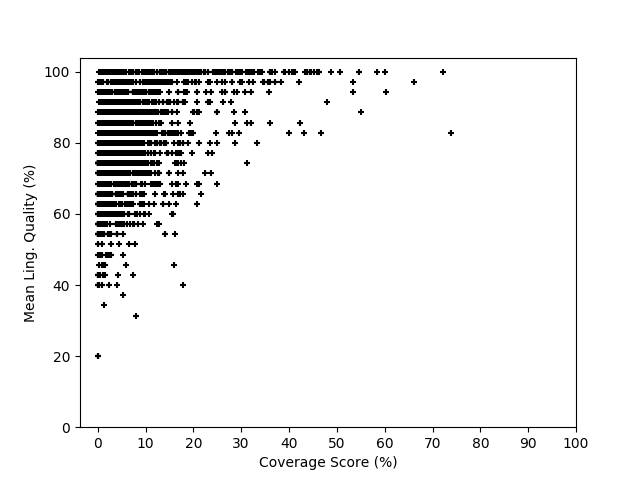
\includegraphics[scale=0.5]{../../my_diagrams/DUC_dataset/scatter_CS_MLQ.png}
\caption{Scatterplot of mean linguistic quality (\textsc{MLQ}) and coverage scores (\textsc{CS}) for human assessments of summaries in DUC-2004.}
\label{graph:scatterplot}
\end{figure}

\begin{figure}[ht]
\centering
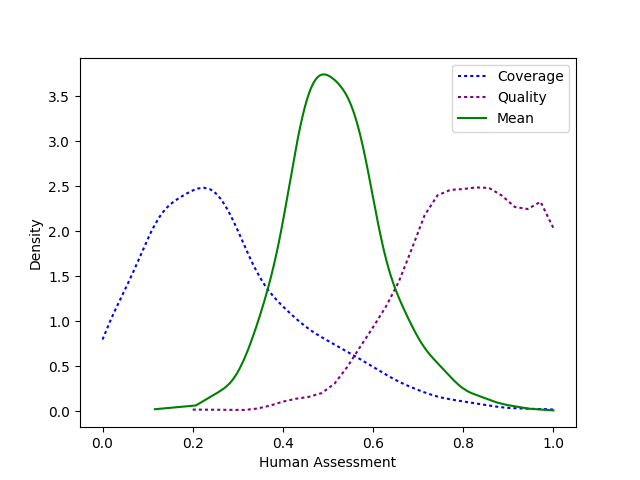
\includegraphics[scale=0.5]{../../my_diagrams/DUC_dataset/density_plots.png}
\caption{Mean linguistic quality (\textsc{MLQ}) and coverage scores (\textsc{CS}) distributions, with the average of the two distributions.}
\label{graph:density}
\end{figure}

\subsection{\bioasq}
\label{ssec:bioasq}

\bioasq is a challenge on biomedical semantic indexing question answering. The challenge 
consists of two tasks, A and B. Task A examines large scale biomedical semantic indexing, 
while Task B examines biomedical semantic QA \cite{Tsatsaronis:2015}. 

Task B examines the ability of systems to annotate questions with concepts from 
relevant ontologies and return either “exact” or paragraph sized “ideal” answers. 
It is organised in two phases, A and B. In Phase A the \bioasq team released questions 
and the systems had to respond with relevant terminological and ontological concepts, 
relevant articles, snippets and RDF snippets. In Phase B, the \bioasq team released questions 
and “gold” (correct) relevant concepts, articles, snippets and statements. The participating 
systems had to respond with “ideal” answers (i.e., paragraph sized summaries) for all 
questions, among other, irrelevant to this article types of responses. The answers are 
called “ideal” since they are what a human would expect from a biomedical expert. In this 
article, we focus on the evaluation of Phase B in Task B.

The dataset was created by the \bioasq team of biomedical experts, and the “gold” 
relevant documents were identified using PUBMED. We used the dataset released for 
the fourth year of the challenge. It consists of 1625 questions and was split into 
a training,  development and test set of 673, 279 and 673 instances respectively 
(after tokenization and stop word removal)(Tables \ref{tab:bioasq_stats_1} and \ref{tab:bioasq_stats_2}). For each 
question in each set a number of system answers is available, and for each system 
answer its human assessment.

Human assessment was provided by the \bioasq team of experts, who inspected 
each system's “ideal” answer and were asked to evaluate it in terms of information
recall (whether the answer contains all the necessary information), information 
precision (whether it contains no irrelevant information), information repetition 
(it does not repeat the same information) and readability (it is easily readable and fluent). 
The criteria were measured in a scale from 1 to 5, with 1 being the worst and 5 the best.

In contrast to the Graham paper, we try to predict the human-assigned
score for each of the aforementioned measures by itself instead of combining
them all to one.

\begin{table}[]
{
\scriptsize
\centering
\begin{tabular}{@{}ccccc@{}}
\toprule
\multicolumn{1}{l}{} & \# questions & \begin{tabular}[c]{@{}c@{}}max \#\\ systems / \\ question\end{tabular} & \begin{tabular}[c]{@{}c@{}}min \#\\ systems / \\ question\end{tabular} & \begin{tabular}[c]{@{}c@{}}mean \#\\ systems / \\ question\end{tabular} \\ \midrule
\begin{tabular}[c]{@{}c@{}}Training \\ set\end{tabular} & 673 & 26 & 2 & 11.6 \\ \midrule
\begin{tabular}[c]{@{}c@{}}Development\\ set\end{tabular} & 279 & 20 & 4 & 10.1 \\ \midrule
\begin{tabular}[c]{@{}c@{}}Test\\ set\end{tabular} & 257 & 17 & 3 & 10 \\ \bottomrule
\end{tabular}
}
\caption{Overview of questions and systems per question for the \bioasq datasets.}
\label{tab:bioasq_stats_1}
\end{table}

\begin{table}[]
{
\scriptsize
\centering
\begin{tabular}{@{}ccccc@{}}
\toprule
\multicolumn{1}{l}{} & \begin{tabular}[c]{@{}c@{}}\# input\\ vectors\end{tabular} & \begin{tabular}[c]{@{}c@{}}mean question\\ length\end{tabular} & \begin{tabular}[c]{@{}c@{}}mean gold\\ answer length\end{tabular} & \begin{tabular}[c]{@{}c@{}}mean system\\ answer length\end{tabular} \\ \midrule
\begin{tabular}[c]{@{}c@{}}Training \\ set\end{tabular} & 7842 & 66.3 & 317.4 & 716.8 \\ \midrule
\begin{tabular}[c]{@{}c@{}}Development\\ set\end{tabular} & 2825 & 64 & 334 & 735 \\ \midrule
\begin{tabular}[c]{@{}c@{}}Test\\ set\end{tabular} & 2574 & 70.2 & 410.3 & 769 \\ \bottomrule
\end{tabular}
}
\caption{Overview of questions and systems per question for the \bioasq datasets.}
\label{tab:bioasq_stats_2}
\end{table}

\section{Methods}
\label{sect:methods}

We will now overview the proposed methods. We attempt to build deep 
\mlp networks to predict the human assessment of the summaries. 
We employ different strategies when handling the inputs, which is 
discussed in the following sections, but the process of determining 
the architecture of the networks is common regardless of their input.

In the \bioasq dataset, we attempted to infer the  human-assigned scores 
to each of the Recall, Precision, Readability and Repetition measures, 
on summaries from the fourth year of the competition.

Having four measures to predict, we experimented with both single and multi-task 
learning . In the single task approach, we define a network which tries to 
predict a single measure’s score at a time (\srouge and \scent, depending on 
the inputs). Thus we end up with four networks, one for each measure and each 
one is optimized to predict the corresponding measure.

In the multi-task approach, for each measure we develop a network which predicts 
the scores for all four measures at the same time. We chose network 
configurations dependant on a specific measure out of the four, again 
ending up with four different networks. We attempt to exploit shared information 
across all four measures so that the predictive capability for a single 
measure can be boosted (\mrouge and \mcent, depending on the inputs).

To build the networks, we followed a common approach for both the single and multi-task
learning strategies. The process consisted of defining different depth and widths for
the architecture, overfitting them on training data and then regularizing the 
architecture which achieved the lowest Mean Squared Error (\textsc{MSE})
loss during overfitting. During regularization, we added dropout layers and 
randomly assigned their rate, as well as randomly assigning values for the L2 penalty 
on the weights. Furthermore, we employed early stopping during training while 
monitoring the loss on the validation data. We used the Adam optimizer with 
learning rate $lr$ = 0.001(\cite{Kingma:2014}).

In the case of \duc the target of the model is \has, the combinatorial measure which 
takes into account the coverage expressed by the system summary, as well as the linguistic 
quality of the system summaries, as annotated by human assessors.

Since the target score in this dataset is a single score, we follow a single task learning 
approach. The methodology used to define this network is identical to the one described in 
the single task learning approach for \bioasq, as are the overfitting and regularization of 
the networks.

\subsection{Deep \mlp over \rouge variations (\srouge \& \mrouge)}
\label{ssec:rouge}

One method we employed was inspired by previous analysis of current evaluation 
methodologies applied to summarization techniques. Graham et al. \shortcite{Graham:2015}
evaluated the performance of different variations of \rouge metrics on 
the \duc dataset. The results suggested that certain variations were much superior 
to others, and the best performing were not always the ones most commonly used. In 
this thesis we attempt to continue this analysis by combining all the metric variations, 
taking advantage of the different insights each of them provides in summarization evaluation.

The \rouge metrics we used include 8 choices of n-gram counting methods (\rouge-1;2;3;4;S4;SU4;W;L), 
binary settings such as word stemming of summaries and inclusion or removal of stop 
words, as well as the use of recall, precision, or f-score to compute individual 
summary scores. In total we examined 96 variations of \rouge.

In addition to the \rouge variants, we also examine metrics based on similarity between the 
gold and system generated summaries. Each system summary is converted to a dense vector, 
representing the centroid of the word embeddings, which is also weighted by term frequency 
(\textsc{TF}) scores. We call this method \cent, and more specifically \cente when the 
Euclidean and \centc when the Cosine similarity are used to compute the similarity between 
the system summary and the gold (the representation of a gold is computed similarly to a 
system summary) \cite{Brokos:2016}.

We also use 6 different variations of Word Mover's Disctance (\wmd). \wmd measures the total 
distance the word embeddings of two summaries have to travel to become identical \cite{Kusner:2015}. 
In the same paper, they introduced a relaxed, faster version of \wmd which measures the 
distance the word embeddings of only one summary have to travel. This led to two different 
Relaxed \wmd (\rwmd) variations according to whether the “left” (\rwmdl) or the “right” 
(\rwmdr) summary's distance from the other was measured, in terms of how many words of 
one are present in the other. They found that the maximum (\rwmdmax) of the two distances 
was the better relaxation. Finally, we differentiate between the use of Euclidean (\rwmde) 
and Cosine (\rwmdc) distance as the metric of choice to use in \rwmd.

The \bleu scores were computed using the \jbleu library.

In total, we calculated 105 metric variations for each system summary. A list of these metrics 
was used as input to each of the deep \mlp architectures described above.

\begin{figure}[ht]
{
\centering
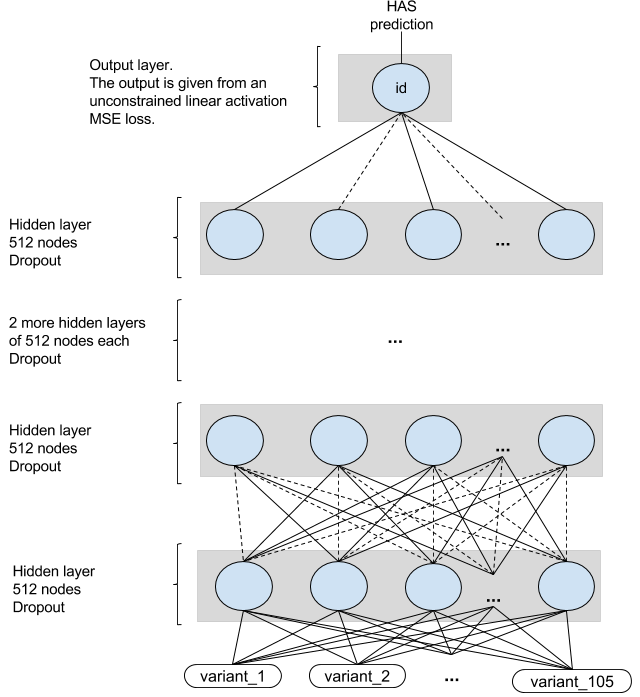
\includegraphics[scale=0.35]{../../my_diagrams/DUC_dataset/DUC_s-rouge.png}
\caption{\textsc{s-rouge} network used on the \duc dataset. The network is 5 layers deep with each layer consisting of 512 nodes.}
\label{fig:duc-srouge}
}
\end{figure}

\begin{figure}[ht]
{
\centering
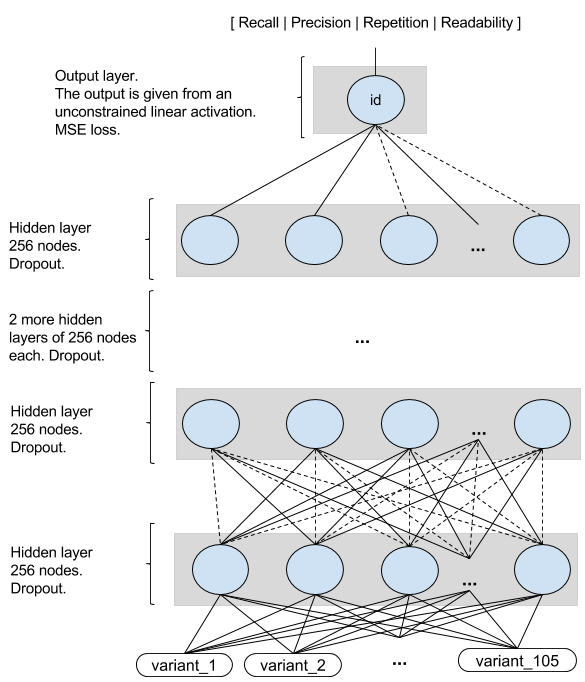
\includegraphics[scale=0.35]{../../my_diagrams/BioASQ_networks/BioASQ-s-rouge.png}
\caption{\textsc{s-rouge} network used on the \bioasq dataset. The network is 5 layers deep with each layer consisting of 256 nodes.}
\label{fig:bioasq-s-rouge}
}
\end{figure}

\begin{figure}[ht]
{
\centering
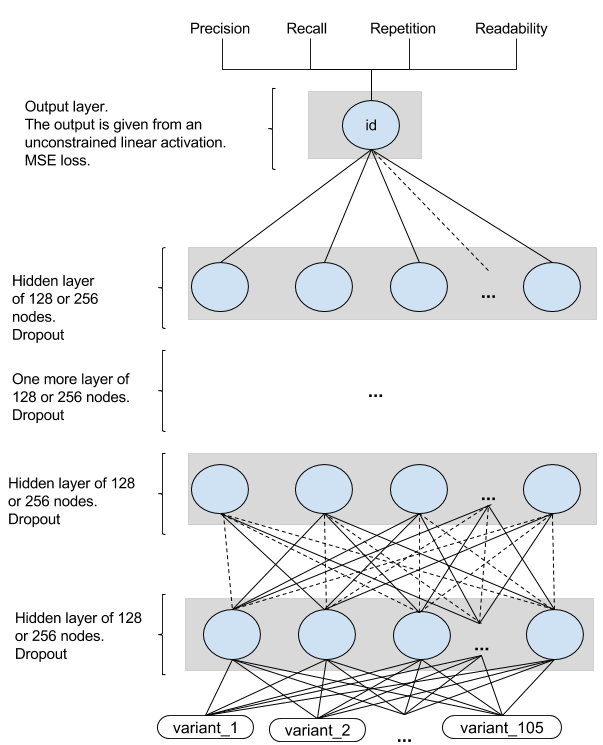
\includegraphics[scale=0.35]{../../my_diagrams/BioASQ_networks/BioASQ-m_rouge.png}
\caption{\textsc{m-rouge} network used on the \bioasq dataset. The exact network architecture depends on the metric, since we create one network for each metric. It can be up to 4 layers deep with each layer consisting of 128 or 256 nodes.}
\label{fig:bioasq-m-rouge}
}
\end{figure}

\subsection{Deep \mlp over difference of centroids (\scent \& \mcent)}
\label{ssec:centroids}

\rouge has a number of limitations which is the motivation for the development 
of the following two methods.

Those limitations have to do both with its implementation and the underlying 
assumptions. \rouge has a large number of variants, of which only a small range 
is commonly used. We include 96 in this study, and depending on the task that 
number can grow. Furthermore, the n-gram coverage of the summaries, as used by 
classic \rouge, favors lexical similarities between the system and human sentences, 
making it unsuitable for evaluating abstractive summaries, or summaries with a 
significant amount of paraphrasing. Finally, It is not suitable for evaluating the 
readability or repetition of the system generated summaries.

In an attempt to combat those limitations we propose the use of the centroid of 
the summaries' word embeddings, instead of relying on the bag-of-words representation. 
While previous work has explored the use of dense representations of words or short 
sequences of words in \rouge with good results \cite{Ng:2015}, no one has made use of
dense representations of whole summaries in the evaluation process to our knowledge.

This method has the advantage of bypassing the need to decide between a large number 
of \rouge variants and the uncertainty this choice entails, while also overcoming any 
bias towards lexical similarity and instead focusing on semantic similarity.

Having a sentence $t$, the centroid representation of that sentence $\vec{t}$ is the 
sum of the embeddings of the tokens in the sentence, divided by the number of the 
tokens in it. In our experiments, we also take into account the $\idf$ scores of 
the tokens:

\begin{align}
\vec{t} = \frac{\sum_{j=1}^{|V|}\vec{w}_j \cdot TF(w_j, t) \cdot IDF(w_j)}{\sum_{j=1}^{|V|} TF(w_j, t) \cdot IDF(w_j)}
\end{align}

where $|V|$ is the vocabulary size (approx. 1.7 million words, ignoring stop words), 
$w_j$ is the $j$-th vocabulary word, $\vec{w}_j$ its embedding, $TF(w_j, t)$ the term 
frequency of $w_j$ in $t$, and $IDF(w_j)$ the inverse document frequency of $w_j$ 
\cite{Manning:2008}.

We use 200-dimensional embeddings and pre-compute the centroid representation of the 
sentences before using them in our models, resulting in 200-dimensional vectors.

In the case of \bioasq, the word embeddings used come from applying \wordvec to 
approximately 11 million abstracts obtained from PubMed. The \idf scores are calculated 
on the vocabulary of those abstracts. In the case of \duc, the word embeddings were 
obtained from the Wikipedia 2015 + Gigaword 5 GloVe repository and the \idf scores 
are computed on the vocabulary of the dataset.

Having computed the centroids of each human and system summary, we subtract the system 
summary centroid representation from the human one and we use the resulting 200-dimensional 
vector as input to each of the deep \mlp architectures described above.

\begin{figure}[ht]
{
\centering
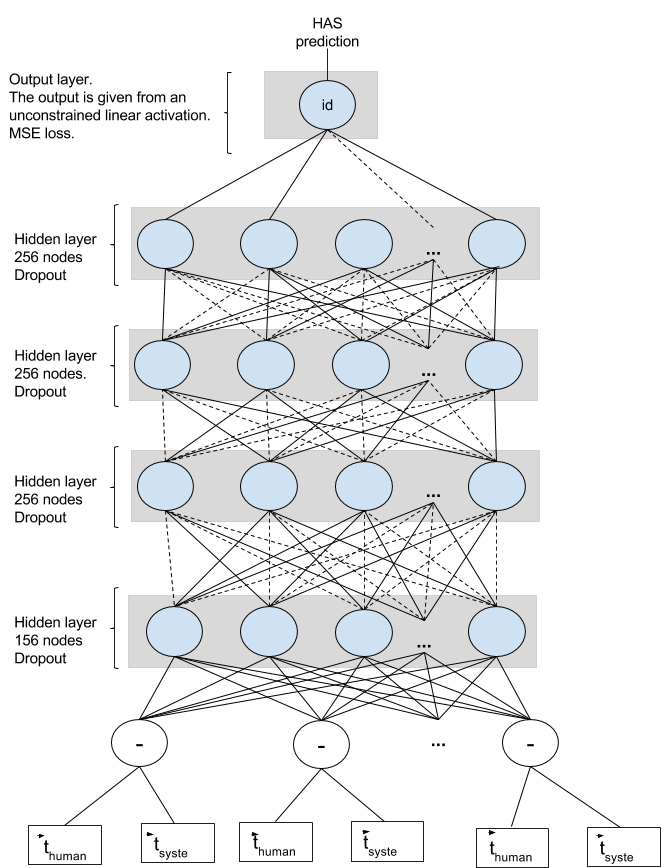
\includegraphics[scale=0.35]{../../my_diagrams/DUC_dataset/DUC_s-cent.png}
\caption{\textsc{s-cent} network used on the \duc dataset, with the difference of the centroids of the summaries as input. The network consists of 4 layers of 256 nodes each.}
\label{fig:duc-s-cent}
}
\end{figure}

\begin{figure}[ht]
{
\centering
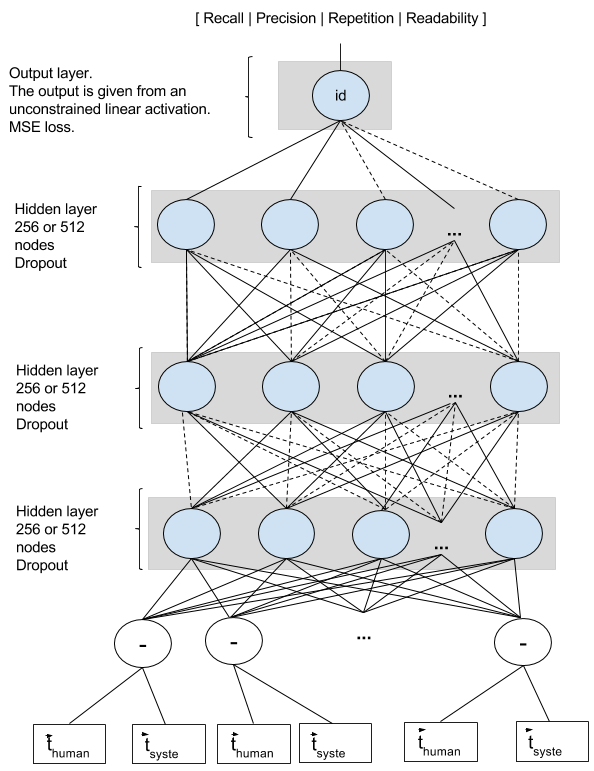
\includegraphics[scale=0.35]{../../my_diagrams/BioASQ_networks/BioASQ_s-cent.png}
\caption{\textsc{s-cent} network used on the \bioasq dataset, with the difference of the centroids of the summaries as input. The exact network architecture depends on the metric, since we create one network for each metric. Each network is 3 layers deep, and each layer consists of 256 or 512 nodes.}
\label{fig:bioasq-s-cent}
}
\end{figure}

\begin{figure}[ht]
{
\centering
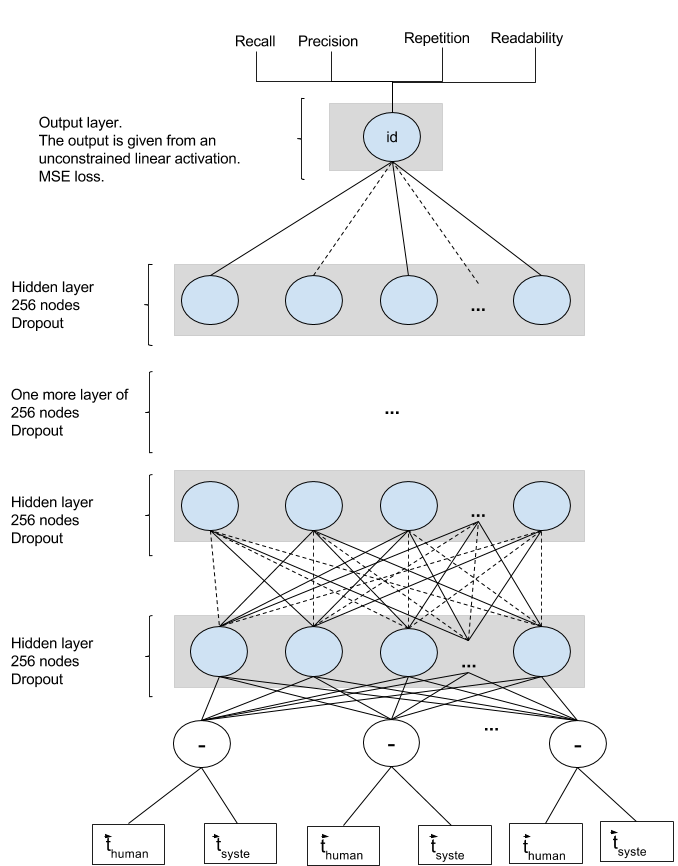
\includegraphics[scale=0.35]{../../my_diagrams/BioASQ_networks/BioASQ_m-cent.png}
\caption{\textsc{m-cent} network used on the \bioasq dataset, with the difference of the centroids of the summaries as input. The exact network architecture depends on the metric, since we create one network for each metric. Each network is up to 5 layers deep, and each layer consists of 256 nodes.}
\label{fig:bioasq-m-cent}
}
\end{figure}


\section{Results}
\label{sec:results}

\subsection{Metric Evaluation by Correlation}
\label{ssec:correlation}

We present correlation results between the human evaluation values and the metric 
values, for both the datasets, for every metric mentioned in this paper. These 
metrics include the 96 \rouge variants, the 2 centroid distance based metrics, 
the 6 variants of \wmd, \bleu and the 4 \mlp metrics we developed.

The performance evaluation for all the metrics was calculated by employing three 
different correlation measures, Pearson's $r$, Spearman's $\rho$ and Kendall's $\tau$. 
All three metrics have been used to explore the correlation between summaries in 
the field of NLP, but there are differences between them.

Pearson correlation estimates linear correlations under the assumption of normally 
distributed data. Spearman correlation estimates the monotonic relationship between 
two datasets, but it does not assume that they are normally distributed. On the other hand, 
Kendall's $\tau$ is a probabilistic function, measuring the discrepancy between the number 
of concordant and discordant pairs. We decided to present the results sorted by Spearman's $\rho$, 
with the two other correlations presented for a complete overview.


\subsection{Metric Significance Testing}
\label{ssec:significance}

The superiority of one metric over another should be examined through significance testing. 
Graham et al, 2015, employed Williams tests to determine the significance of a metric when 
compared with all the other metrics. We are using the same methodology of applying Williams 
tests to the difference between the correlations of measures, instead of exploring the 
significance of each metric on its own. The test can determine whether the metric under 
examination is statistically more  significant than any other, worse performing metric.
In the results tables, a  $\bullet$ next to the Spearman's $\rho$ value indicates that 
the particular metric is not significantly outperformed by any other metric that comes after it.

\subsection{Summarization Metrics Evaluation}
\label{ssec:evaluation}

Table \ref{tab:duc_correlations} shows the correlations of each metric with human assessment 
on the \duc datasets. The \srouge metric was defined in section \ref{ssec:rouge} as the 
single task learning approach to a deep \mlp architecture over an input of all the \rouge 
and other variants. This metric achieves the strongest Spearman correlation value, $\rho$ = 0.624, 
with the human assessment data. The metric also achieves the strongest Pearson's $r$ and 
Kendall's $\tau$, but it does not achieve statistical significance. The next best metric 
is \rouge-2 recall with the words stemmed and stopwords removed, and it is statistically 
significant in this case. This \rouge-1 metric is not among the best metrics as examined 
by Graham et al. \shortcite{Graham:2015}, but \rouge-1 is recommended in Owczarzak et al. \shortcite{Owczarzak:2012}.

\begin{table*}[]
\centering
{
\scriptsize
\begin{tabular}{lllllllllllllll}
\hline
\multicolumn{1}{c}{Metrics} & \multicolumn{1}{c}{Stem.} & \multicolumn{1}{c}{RWS} & \multicolumn{1}{c}{P/R/F} & \multicolumn{1}{c}{$r$} & \multicolumn{1}{c}{$\rho$} & \multicolumn{1}{c}{$\tau$} & \multicolumn{1}{c}{} & \multicolumn{1}{c}{Metrics} & \multicolumn{1}{c}{Stem.} & \multicolumn{1}{c}{RWS} & \multicolumn{1}{c}{P/R/F} & \multicolumn{1}{c}{$r$} & \multicolumn{1}{c}{$\rho$} & \multicolumn{1}{c}{$\tau$} \\ \hline
\textsc{S-ROUGE} & - & - & - & 0.651 & 0.624 & 0.456 &  & \textsc{R-L} & N & N & P & 0.587 & 0.479 & 0.332 \\
\textsc{R-1} & Y & Y & R & 0.647 & 0.602 $\bullet$ & 0.433 &  & \textsc{R-L} & Y & Y & R & 0.589 & 0.474 & 0.332 \\
\textsc{R-1} & Y & Y & F1 & 0.628 & 0.571 & 0.409 &  & \textsc{R-2} & N & N & R & 0.591 & 0.474 & 0.325 \\
\textsc{R-W} & Y & Y & P & 0.616 & 0.552 & 0.389 &  & \textsc{R-3} & Y & Y & R & 0.592 & 0.473 & 0.337 \\
\textsc{R-3} & Y & N & R & 0.605 & 0.551 & 0.395 &  & \textsc{R-4} & N & N & R & 0.532 & 0.467 & 0.350 \\
\textsc{R-3} & Y & N & F1 & 0.606 & 0.549 & 0.392 &  & \textsc{R-4} & N & N & F1 & 0.532 & 0.465 & 0.348 \\
\textsc{R-S4} & Y & Y & R & 0.608 & 0.548 & 0.392 &  & \textsc{R-W} & N & N & F1 & 0.576 & 0.465 & 0.321 \\
\textsc{R-W} & Y & N & P & 0.605 & 0.547 & 0.386 &  & \textsc{R-L} & Y & N & R & 0.589 & 0.464 & 0.320 \\
\textsc{R-3} & Y & N & P & 0.607 & 0.546 & 0.389 &  & \textsc{R-4} & N & N & P & 0.532 & 0.463 & 0.345 \\
\textsc{R-S4} & Y & Y & F1 & 0.609 & 0.545 & 0.388 &  & \textsc{R-4} & N & Y & P & 0.449 & 0.463 & 0.358 \\
\textsc{R-2} & Y & N & F1 & 0.628 & 0.543 & 0.386 &  & \textsc{R-4} & N & Y & F1 & 0.448 & 0.462 & 0.358 \\
\textsc{R-L} & Y & Y & P & 0.616 & 0.541 & 0.380 &  & \textsc{R-4} & N & Y & R & 0.446 & 0.462 & 0.359 \\
\textsc{R-2} & Y & Y & R & 0.625 & 0.539 & 0.385 &  & \textsc{rwmd-r-c} & - & - & - & 0.441 & 0.455 & 0.314 \\
\textsc{R-2} & Y & N & P & 0.626 & 0.537 & 0.380 &  & \textsc{R-4} & Y & Y & P & 0.576 & 0.452 & 0.338 \\
\textsc{R-W} & Y & N & F1 & 0.597 & 0.536 & 0.378 &  & \textsc{R-4} & Y & Y & F1 & 0.577 & 0.451 & 0.339 \\
\textsc{R-2} & Y & Y & F1 & 0.624 & 0.535 & 0.380 &  & \textsc{R-4} & Y & Y & R & 0.577 & 0.444 & 0.334 \\
\textsc{R-1} & Y & N & F1 & 0.622 & 0.534 & 0.378 &  & \textsc{R-3} & N & Y & F1 & 0.496 & 0.443 & 0.335 \\
\textsc{R-S4} & Y & Y & P & 0.607 & 0.533 & 0.378 &  & \textsc{R-1} & N & Y & F1 & 0.523 & 0.442 & 0.306 \\
\textsc{R-SU4} & Y & Y & R & 0.606 & 0.533 & 0.379 &  & \textsc{R-3} & N & Y & P & 0.495 & 0.442 & 0.333 \\
\textsc{R-2} & Y & N & R & 0.626 & 0.533 & 0.378 &  & \textsc{R-L} & N & N & F1 & 0.576 & 0.442 & 0.302 \\
\textsc{R-SU4} & Y & Y & F1 & 0.606 & 0.532 & 0.379 &  & \textsc{R-2} & N & Y & F1 & 0.540 & 0.440 & 0.315 \\
\textsc{rwmd-l-e} & - & - & - & 0.544 & 0.529 & 0.372 &  & \textsc{R-3} & N & Y & R & 0.495 & 0.437 & 0.330 \\
\textsc{R-W} & Y & Y & F1 & 0.606 & 0.527 & 0.371 &  & \textsc{R-S4} & N & N & P & 0.574 & 0.436 & 0.300 \\
\textsc{R-L} & Y & N & P & 0.614 & 0.527 & 0.372 &  & \textsc{R-2} & N & Y & P & 0.525 & 0.436 & 0.310 \\
\textsc{rwmd-l-c} & - & - & - & 0.532 & 0.526 & 0.366 &  & \textsc{R-SU4} & N & N & P & 0.574 & 0.435 & 0.299 \\
\textsc{R-S4} & Y & N & P & 0.612 & 0.525 & 0.369 &  & \textsc{R-SU4} & N & Y & P & 0.535 & 0.433 & 0.300 \\
\textsc{rwmd-m-c} & - & - & - & 0.525 & 0.523 & 0.365 &  & \textsc{R-S4} & N & Y & P & 0.535 & 0.433 & 0.300 \\
\textsc{R-SU4} & Y & Y & P & 0.605 & 0.523 & 0.370 &  & \textsc{R-S4} & N & Y & F1 & 0.537 & 0.432 & 0.299 \\
\textsc{R-SU4} & Y & N & P & 0.610 & 0.520 & 0.366 &  & \textsc{R-SU4} & N & Y & F1 & 0.538 & 0.431 & 0.299 \\
\textsc{rwmd-m-e} & - & - & - & 0.541 & 0.520 & 0.362 &  & \textsc{R-2} & N & Y & R & 0.543 & 0.431 & 0.309 \\
\textsc{R-S4} & Y & N & F1 & 0.610 & 0.519 & 0.366 &  & \textsc{rwmd-r-e} & - & - & - & 0.431 & 0.426 & 0.294 \\
\textsc{R-SU4} & Y & N & F1 & 0.609 & 0.515 & 0.362 &  & \textsc{R-SU4} & N & Y & R & 0.537 & 0.425 & 0.295 \\
\textsc{R-L} & Y & Y & F1 & 0.604 & 0.515 & 0.361 &  & \textsc{R-S4} & N & Y & R & 0.537 & 0.425 & 0.296 \\
\textsc{R-1} & Y & N & P & 0.597 & 0.515 & 0.364 &  & \textsc{BLEU} & - & - & - & 0.417 & 0.424 & 0.295 \\
\textsc{R-1} & Y & Y & P & 0.576 & 0.514 & 0.364 &  & \textsc{R-W} & N & N & R & 0.563 & 0.422 & 0.287 \\
\textsc{R-1} & Y & N & R & 0.605 & 0.513 & 0.362 &  & \textsc{R-S4} & N & N & F1 & 0.573 & 0.421 & 0.289 \\
\textsc{R-2} & Y & Y & P & 0.614 & 0.512 & 0.361 &  & \textsc{R-SU4} & N & N & F1 & 0.573 & 0.421 & 0.289 \\
\textsc{R-3} & N & N & R & 0.564 & 0.508 & 0.369 &  & \textsc{R-1} & N & N & P & 0.522 & 0.416 & 0.288 \\
\textsc{R-3} & N & N & P & 0.563 & 0.508 & 0.368 &  & \textsc{R-1} & N & N & F1 & 0.528 & 0.410 & 0.282 \\
\textsc{R-3} & N & N & F1 & 0.564 & 0.508 & 0.368 &  & \textsc{R-W} & N & Y & P & 0.542 & 0.410 & 0.278 \\
\textsc{R-S4} & Y & N & R & 0.608 & 0.504 & 0.356 &  & \textsc{R-S4} & N & N & R & 0.569 & 0.407 & 0.278 \\
\textsc{R-L} & Y & N & F1 & 0.603 & 0.503 & 0.352 &  & \textsc{R-SU4} & N & N & R & 0.569 & 0.407 & 0.278 \\
\textsc{R-SU4} & Y & N & R & 0.606 & 0.499 & 0.352 &  & \textsc{CENT-C} & - & - & - & 0.348 & 0.404 & 0.276 \\
\textsc{R-4} & Y & N & R & 0.588 & 0.498 & 0.365 &  & \textsc{R-L} & N & N & R & 0.562 & 0.402 & 0.273 \\
\textsc{R-W} & Y & N & R & 0.590 & 0.498 & 0.346 &  & \textsc{R-L} & N & Y & P & 0.544 & 0.401 & 0.273 \\
\textsc{R-W} & N & N & P & 0.584 & 0.496 & 0.343 &  & \textsc{R-1} & N & Y & P & 0.491 & 0.400 & 0.273 \\
\textsc{R-4} & Y & N & F1 & 0.588 & 0.496 & 0.362 &  & \textsc{R-1} & N & N & R & 0.486 & 0.388 & 0.265 \\
\textsc{R-4} & Y & N & P & 0.588 & 0.495 & 0.360 &  & \textsc{R-W} & N & Y & F1 & 0.537 & 0.384 & 0.261 \\
\textsc{R-2} & N & N & P & 0.587 & 0.491 & 0.338 &  & \textsc{R-L} & N & Y & F1 & 0.538 & 0.378 & 0.257 \\
\textsc{R-1} & N & Y & R & 0.547 & 0.487 & 0.340 &  & \textsc{R-W} & N & Y & R & 0.529 & 0.363 & 0.245 \\
\textsc{R-3} & Y & Y & P & 0.593 & 0.486 & 0.344 &  & \textsc{R-L} & N & Y & R & 0.531 & 0.360 & 0.243 \\
\textsc{R-2} & N & N & F1 & 0.592 & 0.486 & 0.334 &  & \textsc{CENT-E} & - & - & - & 0.323 & 0.347 & 0.236 \\
\textsc{R-3} & Y & Y & F1 & 0.593 & 0.484 & 0.344 &  & \textsc{S-CENT} & - & - & - & 0.293 & 0.282 & 0.187 \\
\textsc{R-W} & Y & Y & R & 0.594 & 0.484 & 0.337 &  &  &  &  &  &  &  &  \\ \hline
\end{tabular}
}
\caption{Pearson ($r$), Spearman ($\rho$) and Kendall ($\tau$) correlations of BLEU, 96 variants 
of \rouge (R-*), centroid distance based metrics (\centc, \cente), \wmd based metrics and 
methods described in this paper(\srouge, \scent) with human assessment in \duc. The \rouge 
variants are presented with (Y) and without (N) stemming, with (Y) and without (N) removal of 
stop words (RSW), aggregated at the summary level using precision (P), recall (R) or f-score (F).
The results are sorted in descending order by $\rho$. Correlations marked with $\bullet$ signify 
a metric/variant whose correlation with human assessment is not significantly weaker than that 
of any other metric/variant according to pairwise Williams significance tests.}
\label{tab:duc_correlations}
\end{table*}

Table \ref{tab:bioasq-repetition-correlations} contains the correlations between each metric 
and the human assigned repetition score in the \bioasq dataset. We see that the \srouge metric 
once again achieves the strongest Spearman correlation, $\rho$ = 0.55, with a significant 
margin from the second best metric, which also holds for the other two correlations. The metric 
is not significantly outperformed by any other metric we examined. The second best correlation 
is \rouge-W precision with stemming and stopwords removed, also not among the recommended 
metrics in the papers of Graham \shortcite{Graham:2015} or Owczarzak \shortcite{Owczarzak:2012}. 
The \rouge variants most sensitive to repetition appear to be those using precision and F1 to 
calculate the individual summary scores, and based on the length of common subsequences 
found in the summaries, which intuitively is expected, especially since the variants that 
are N-gram based do the worst.

\begin{table*}[]
{
\scriptsize
\centering
\begin{tabular}{lllllllllllllll}
\hline
\multicolumn{1}{c}{Metrics} & \multicolumn{1}{c}{Stem.} & \multicolumn{1}{c}{RWS} & \multicolumn{1}{c}{P/R/F} & \multicolumn{1}{c}{$r$} & \multicolumn{1}{c}{$\rho$} & \multicolumn{1}{c}{$\tau$} & \multicolumn{1}{c}{} & \multicolumn{1}{c}{Metrics} & \multicolumn{1}{c}{Stem.} & \multicolumn{1}{c}{RWS} & \multicolumn{1}{c}{P/R/F} & \multicolumn{1}{c}{$r$} & \multicolumn{1}{c}{$\rho$} & \multicolumn{1}{c}{$\tau$} \\ \hline
\textsc{S-ROUGE} & - & - & - & 0.494 & 0.550 $\bullet$ & 0.432 &  & \textsc{R-S4} & N & N & F1 & 0.144 & 0.111 & 0.085 \\
\textsc{R-W} & Y & Y & P & 0.347 & 0.439 $\bullet$ & 0.342 &  & \textsc{R-1} & N & N & F1 & 0.204 & 0.105 & 0.080 \\
\textsc{R-L} & Y & Y & P & 0.373 & 0.434 $\bullet$ & 0.339 &  & \textsc{R-2} & N & N & F1 & 0.131 & 0.097 & 0.075 \\
\textsc{R-W} & Y & N & P & 0.324 & 0.425 & 0.332 &  & \textsc{R-2} & N & Y & F1 & 0.127 & 0.083 & 0.064 \\
\textsc{R-W} & N & Y & P & 0.335 & 0.421 & 0.329 &  & \textsc{R-4} & Y & N & P & 0.166 & 0.079 & 0.064 \\
\textsc{R-L} & Y & N & P & 0.354 & 0.420 & 0.329 &  & \textsc{R-3} & Y & N & F1 & 0.131 & 0.076 & 0.060 \\
\textsc{R-L} & N & Y & P & 0.358 & 0.416 & 0.325 &  & \textsc{R-4} & Y & Y & P & 0.167 & 0.076 & 0.064 \\
\textsc{R-W} & N & N & P & 0.316 & 0.414 & 0.323 &  & \textsc{R-3} & Y & Y & F1 & 0.132 & 0.075 & 0.060 \\
\textsc{R-L} & N & N & P & 0.344 & 0.410 $\bullet$ & 0.320 &  & \textsc{CENT-E} & - & - & - & 0.283 & 0.074 & 0.055 \\
\textsc{R-W} & Y & Y & F1 & 0.299 & 0.347 $\bullet$ & 0.269 &  & \textsc{M-ROUGE} & - & - & - & 0.271 & 0.070 & 0.052 \\
\textsc{R-L} & Y & Y & F1 & 0.321 & 0.337 & 0.261 &  & \textsc{R-3} & N & N & P & 0.157 & 0.068 & 0.054 \\
\textsc{R-W} & Y & N & F1 & 0.281 & 0.337 & 0.261 &  & \textsc{R-4} & Y & Y & F1 & 0.120 & 0.051 & 0.043 \\
\textsc{R-W} & N & Y & F1 & 0.286 & 0.329 & 0.255 &  & \textsc{R-4} & Y & N & F1 & 0.122 & 0.049 & 0.040 \\
\textsc{R-L} & Y & N & F1 & 0.307 & 0.329 & 0.255 &  & \textsc{R-4} & N & Y & P & 0.137 & 0.049 & 0.041 \\
\textsc{R-W} & N & N & F1 & 0.273 & 0.325 & 0.252 &  & \textsc{R-4} & N & N & P & 0.141 & 0.046 & 0.037 \\
\textsc{R-L} & N & N & F1 & 0.298 & 0.319 $\bullet$ & 0.247 &  & \textsc{R-3} & N & Y & P & 0.151 & 0.044 & 0.036 \\
\textsc{R-L} & N & Y & F1 & 0.305 & 0.319 & 0.247 &  & \textsc{R-4} & N & Y & F1 & 0.094 & 0.035 & 0.029 \\
\textsc{rwmd-r-c} & - & - & - & 0.374 & 0.277 & 0.213 &  & \textsc{R-3} & N & N & F1 & 0.109 & 0.033 & 0.026 \\
\textsc{R-1} & Y & Y & P & 0.319 & 0.272 $\bullet$ & 0.209 &  & \textsc{R-4} & N & N & F1 & 0.099 & 0.025 & 0.020 \\
\textsc{rwmd-r-e} & - & - & - & 0.338 & 0.258 & 0.199 &  & \textsc{R-3} & N & Y & F1 & 0.104 & 0.021 $\bullet$ & 0.017 \\
\textsc{R-1} & Y & N & P & 0.308 & 0.250 & 0.193 &  & \textsc{R-4} & N & Y & R & -0.017 & -0.007 & -0.006 \\
\textsc{R-SU4} & Y & Y & P & 0.233 & 0.237 & 0.182 &  & \textsc{R-4} & Y & Y & R & -0.006 & -0.014 $\bullet$ & -0.012 \\
\textsc{R-1} & N & Y & P & 0.279 & 0.236 & 0.182 &  & \textsc{R-4} & Y & N & R & -0.008 & -0.029 & -0.024 \\
\textsc{S-CENT} & - & - & - & 0.43 & 0.233 & 0.179 &  & \textsc{R-4} & N & N & R & -0.024 & -0.033 & -0.028 \\
\textsc{R-SU4} & N & Y & P & 0.224 & 0.222 & 0.171 &  & \textsc{R-3} & Y & Y & R & -0.022 & -0.034 & -0.028 \\
\textsc{R-1} & N & N & P & 0.280 & 0.221 & 0.170 &  & \textsc{R-SU4} & N & Y & R & -0.011 & -0.036 & -0.030 \\
\textsc{BLEU} & - & - & - & 0.191 & 0.219 & 0.168 &  & \textsc{R-3} & Y & N & R & -0.017 & -0.038 & -0.031 \\
\textsc{rwmd-m-c} & - & - & - & 0.341 & 0.219 & 0.169 &  & \textsc{R-SU4} & Y & Y & R & -0.012 & -0.042 & -0.035 \\
\textsc{R-S4} & Y & Y & P & 0.226 & 0.216 $\bullet$ & 0.167 &  & \textsc{R-2} & Y & Y & R & -0.027 & -0.049 & -0.039 \\
\textsc{R-S4} & N & Y & P & 0.218 & 0.205 & 0.158 &  & \textsc{R-3} & N & Y & R & -0.035 & -0.051 & -0.042 \\
\textsc{R-SU4} & Y & N & P & 0.211 & 0.202 & 0.155 &  & \textsc{R-2} & N & Y & R & -0.04 & -0.051 & -0.041 \\
\textsc{R-S4} & Y & N & P & 0.208 & 0.194 & 0.149 &  & \textsc{R-S4} & N & Y & R & -0.025 & -0.051 & -0.041 \\
\textsc{R-2} & Y & N & P & 0.212 & 0.193 & 0.149 &  & \textsc{R-3} & N & N & R & -0.032 & -0.052 & -0.043 \\
\textsc{rwmd-m-e} & - & - & - & 0.300 & 0.190 & 0.146 &  & \textsc{R-2} & Y & N & R & -0.027 & -0.053 & -0.043 \\
\textsc{R-SU4} & N & N & P & 0.205 & 0.190 & 0.146 &  & \textsc{R-2} & N & N & R & -0.038 & -0.055 & -0.044 \\
\textsc{R-2} & Y & Y & P & 0.215 & 0.185 & 0.144 &  & \textsc{R-S4} & Y & Y & R & -0.028 & -0.058 & -0.048 \\
\textsc{R-S4} & N & N & P & 0.202 & 0.183 $\bullet$ & 0.140 &  & \textsc{R-SU4} & N & N & R & -0.025 & -0.066 & -0.054 \\
\textsc{R-2} & N & N & P & 0.187 & 0.157 & 0.122 &  & \textsc{R-SU4} & Y & N & R & -0.028 & -0.070 & -0.057 \\
\textsc{R-SU4} & Y & Y & F1 & 0.168 & 0.155 & 0.118 &  & \textsc{R-S4} & N & N & R & -0.032 & -0.071 & -0.058 \\
\textsc{R-1} & Y & Y & F1 & 0.241 & 0.154 & 0.117 &  & \textsc{R-S4} & Y & N & R & -0.036 & -0.077 & -0.063 \\
\textsc{R-SU4} & N & Y & F1 & 0.162 & 0.147 & 0.112 &  & \textsc{rwmd-l-e} & - & - & - & 0.033 & -0.078 & -0.063 \\
\textsc{R-S4} & Y & Y & F1 & 0.160 & 0.139 & 0.106 &  & \textsc{R-W} & N & Y & R & -0.014 & -0.078 & -0.062 \\
\textsc{M-CENT} & - & - & - & 0.428 & 0.138 & 0.105 &  & \textsc{rwmd-l-c} & - & - & - & 0.140 & -0.078 & -0.063 \\
\textsc{R-1} & N & Y & F1 & 0.207 & 0.134 & 0.102 &  & \textsc{R-W} & Y & Y & R & -0.012 & -0.078 & -0.062 \\
\textsc{R-S4} & N & Y & F1 & 0.155 & 0.133 & 0.101 &  & \textsc{R-W} & N & N & R & -0.017 & -0.084 & -0.067 \\
\textsc{CENT-C} & - & - & - & 0.322 & 0.132 & 0.101 &  & \textsc{R-W} & Y & N & R & -0.016 & -0.085 & -0.069 \\
\textsc{R-2} & N & Y & P & 0.182 & 0.131 & 0.103 &  & \textsc{R-1} & Y & Y & R & 0.038 & -0.092 & -0.074 \\
\textsc{R-1} & Y & N & F1 & 0.232 & 0.127 & 0.096 &  & \textsc{R-1} & N & Y & R & 0.005 & -0.093 & -0.075 \\
\textsc{R-SU4} & Y & N & F1 & 0.151 & 0.122 & 0.093 &  & \textsc{R-L} & N & Y & R & -0.031 & -0.106 $\bullet$ & -0.084 \\
\textsc{R-3} & Y & N & P & 0.182 & 0.122 & 0.097 &  & \textsc{R-L} & Y & Y & R & -0.030 & -0.110 & -0.088 \\
\textsc{R-2} & Y & N & F1 & 0.149 & 0.120 & 0.092 &  & \textsc{R-L} & N & N & R & -0.041 & -0.121 & -0.097 \\
\textsc{R-2} & Y & Y & F1 & 0.148 & 0.116 & 0.089 &  & \textsc{R-1} & Y & N & R & 0.027 & -0.121 & -0.098 \\
\textsc{R-S4} & Y & N & F1 & 0.147 & 0.116 & 0.088 &  & \textsc{R-L} & Y & N & R & -0.042 & -0.126 & -0.101 \\
\textsc{R-SU4} & N & N & F1 & 0.147 & 0.116 & 0.088 &  & \textsc{R-1} & N & N & R & -0.002 & -0.129 & -0.105 \\
\textsc{R-3} & Y & Y & P & 0.184 & 0.113 & 0.091 &  &  &  &  &  &  &  &  \\ \hline
\end{tabular}
}
\caption{Pearson ($r$), Spearman ($\rho$) and Kendall ($\tau$) correlations of BLEU, 96 variants 
of \rouge (R-*), centroid distance based metrics (\centc, \cente), \wmd based metrics and 
methods described in this paper(\srouge, \mrouge, \scent, \mcent) with human assessment of the \textbf{Repetition} metric in \bioasq. The \rouge 
variants are presented with (Y) and without (N) stemming, with (Y) and without (N) removal of 
stop words (RSW), aggregated at the summary level using precision (P), recall (R) or f-score (F).
The results are sorted in descending order by $\rho$. Correlations marked with $\bullet$ signify 
a metric/variant whose correlation with human assessment is not significantly weaker than that 
of any other metric/variant according to pairwise Williams significance tests.}
\label{tab:bioasq-repetition-correlations}
\end{table*}



Table \ref{tab:bioasq-recall-correlations} shows the correlations between each metric and the human 
assigned recall score in \bioasq. The metric that achieves the strongest Spearman correlation 
with $\rho$ = 0.529 is \mrouge which was defined in section \ref{ssec:rouge} as well. In this case, 
it refers to the multitask learning approach to the \mlp architecture with the same input as 
described above. The second best approach with $\rho$ = 0.525 is \srouge. The metrics retain 
their relative position when the other two correlation measures are considered. The absolute 
difference between the $\rho$ values is very small though, and of the two, \srouge is the one 
not significanlty outperformed by any other metric in the list. In terms of \rouge variants, 
the \rouge-W recall with stopword removal comes third in its correlation strength, with significantly 
lower correlation value. Worth noting is that the top \rouge variants in this case are all 
recall based, and based on the longest common subsequence of words present in the summaries, 
whether weighted (\rouge-W) or not (\rouge-L).

\begin{table*}[]
{
\scriptsize
\centering
\begin{tabular}{lllllllllllllll}
\hline
\multicolumn{1}{c}{Metrics} & \multicolumn{1}{c}{Stem.} & \multicolumn{1}{c}{RWS} & \multicolumn{1}{c}{P/R/F} & \multicolumn{1}{c}{$r$} & \multicolumn{1}{c}{$\rho$} & \multicolumn{1}{c}{$\tau$} & \multicolumn{1}{c}{} & \multicolumn{1}{c}{Metrics} & \multicolumn{1}{c}{Stem.} & \multicolumn{1}{c}{RWS} & \multicolumn{1}{c}{P/R/F} & \multicolumn{1}{c}{$r$} & \multicolumn{1}{c}{$\rho$} & \multicolumn{1}{c}{$\tau$} \\ \hline
\textsc{M-ROUGE} & - & - & - & 0.584 & 0.529 & 0.417 &  & \textsc{R-2} & N & N & F1 & 0.266 & 0.321 & 0.252 \\
\textsc{S-ROUGE} & - & - & - & 0.531 & 0.525 $\bullet$ & 0.413 &  & \textsc{R-4} & Y & Y & R & 0.287 & 0.320 & 0.267 \\
\textsc{R-W} & N & Y & R & 0.452 & 0.502 & 0.396 &  & \textsc{R-2} & N & Y & F1 & 0.256 & 0.313 & 0.248 \\
\textsc{R-W} & Y & Y & R & 0.458 & 0.499 $\bullet$ & 0.394 &  & \textsc{R-3} & Y & N & P & 0.199 & 0.313 & 0.249 \\
\textsc{R-W} & N & N & R & 0.434 & 0.487 & 0.383 &  & \textsc{R-1} & Y & N & F1 & 0.368 & 0.312 & 0.242 \\
\textsc{R-L} & N & Y & R & 0.466 & 0.486 & 0.384 &  & \textsc{R-1} & N & Y & F1 & 0.345 & 0.310 & 0.241 \\
\textsc{R-W} & Y & N & R & 0.437 & 0.484 & 0.381 &  & \textsc{R-2} & Y & Y & P & 0.233 & 0.309 & 0.242 \\
\textsc{R-L} & Y & Y & R & 0.471 & 0.483 $\bullet$ & 0.382 &  & \textsc{R-SU4} & N & Y & P & 0.22 & 0.307 & 0.238 \\
\textsc{R-L} & N & N & R & 0.449 & 0.467 & 0.368 &  & \textsc{R-4} & Y & N & F1 & 0.227 & 0.302 & 0.246 \\
\textsc{rwmd-l-e} & - & - & - & 0.471 & 0.465 & 0.369 &  & \textsc{R-S4} & N & Y & P & 0.215 & 0.301 & 0.234 \\
\textsc{R-L} & Y & N & R & 0.451 & 0.464 & 0.366 &  & \textsc{R-4} & N & N & R & 0.266 & 0.297 & 0.250 \\
\textsc{rwmd-l-c} & - & - & - & 0.541 & 0.454 & 0.360 &  & \textsc{rwmd-m-e} & - & - & - & 0.342 & 0.296 & 0.230 \\
\textsc{R-SU4} & Y & Y & R & 0.394 & 0.448 & 0.352 &  & \textsc{R-3} & Y & Y & P & 0.199 & 0.296 & 0.238 \\
\textsc{R-SU4} & N & Y & R & 0.382 & 0.444 & 0.348 &  & \textsc{rwmd-m-c} & - & - & - & 0.396 & 0.295 & 0.228 \\
\textsc{R-S4} & Y & Y & R & 0.391 & 0.439 & 0.345 &  & \textsc{R-2} & Y & N & P & 0.223 & 0.293 & 0.228 \\
\textsc{R-2} & Y & Y & R & 0.395 & 0.438 & 0.347 &  & \textsc{R-SU4} & Y & Y & P & 0.220 & 0.292 & 0.226 \\
\textsc{R-2} & Y & N & R & 0.395 & 0.434 & 0.342 &  & \textsc{R-3} & N & N & F1 & 0.226 & 0.292 & 0.237 \\
\textsc{R-S4} & N & Y & R & 0.378 & 0.433 & 0.340 &  & \textsc{R-4} & Y & Y & F1 & 0.220 & 0.289 & 0.239 \\
\textsc{R-1} & Y & Y & R & 0.481 & 0.431 & 0.340 &  & \textsc{R-S4} & Y & Y & P & 0.216 & 0.286 & 0.222 \\
\textsc{R-SU4} & Y & N & R & 0.379 & 0.420 & 0.329 &  & \textsc{R-4} & Y & N & P & 0.176 & 0.281 & 0.229 \\
\textsc{R-S4} & Y & N & R & 0.379 & 0.418 & 0.328 &  & \textsc{R-3} & N & Y & R & 0.270 & 0.281 & 0.235 \\
\textsc{R-SU4} & N & N & R & 0.371 & 0.417 & 0.326 &  & \textsc{R-4} & N & Y & R & 0.230 & 0.277 & 0.237 \\
\textsc{R-1} & Y & N & R & 0.470 & 0.415 & 0.327 &  & \textsc{R-1} & N & N & F1 & 0.325 & 0.273 & 0.212 \\
\textsc{R-S4} & N & N & R & 0.370 & 0.414 $\bullet$ & 0.324 &  & \textsc{CENT-E} & - & - & - & 0.398 & 0.271 & 0.210 \\
\textsc{R-3} & Y & N & R & 0.343 & 0.394 & 0.315 &  & \textsc{R-4} & N & N & F1 & 0.199 & 0.271 & 0.227 \\
\textsc{R-1} & N & Y & R & 0.423 & 0.383 & 0.300 &  & \textsc{R-SU4} & N & N & P & 0.207 & 0.270 & 0.209 \\
\textsc{R-2} & N & N & R & 0.352 & 0.383 & 0.303 &  & \textsc{R-2} & N & Y & P & 0.196 & 0.268 & 0.212 \\
\textsc{R-W} & N & Y & F1 & 0.299 & 0.379 & 0.295 &  & \textsc{R-4} & Y & Y & P & 0.174 & 0.267 & 0.221 \\
\textsc{R-2} & N & Y & R & 0.337 & 0.374 & 0.298 &  & \textsc{R-3} & N & N & P & 0.173 & 0.267 & 0.217 \\
\textsc{R-1} & N & N & R & 0.425 & 0.373 & 0.293 &  & \textsc{R-S4} & N & N & P & 0.203 & 0.266 & 0.206 \\
\textsc{R-3} & Y & Y & R & 0.333 & 0.372 & 0.301 &  & \textsc{R-2} & N & N & P & 0.195 & 0.260 & 0.204 \\
\textsc{CENT-C} & - & - & - & 0.487 & 0.371 & 0.290 &  & \textsc{R-SU4} & Y & N & P & 0.206 & 0.260 & 0.201 \\
\textsc{R-W} & Y & Y & F1 & 0.300 & 0.370 & 0.288 &  & \textsc{R-4} & N & Y & F1 & 0.182 & 0.257 & 0.219 \\
\textsc{R-W} & N & N & F1 & 0.285 & 0.370 & 0.288 &  & \textsc{R-S4} & Y & N & P & 0.202 & 0.256 & 0.198 \\
\textsc{R-2} & Y & Y & F1 & 0.305 & 0.369 & 0.288 &  & \textsc{R-4} & N & N & P & 0.153 & 0.256 & 0.214 \\
\textsc{R-SU4} & N & Y & F1 & 0.284 & 0.369 & 0.287 &  & \textsc{R-1} & Y & Y & P & 0.284 & 0.252 & 0.194 \\
\textsc{BLEU} & - & - & - & 0.229 & 0.368 & 0.287 &  & \textsc{R-3} & N & Y & F1 & 0.208 & 0.251 & 0.208 \\
\textsc{R-2} & Y & N & F1 & 0.302 & 0.365 & 0.285 &  & \textsc{R-4} & N & Y & P & 0.148 & 0.245 & 0.208 \\
\textsc{R-W} & Y & N & F1 & 0.285 & 0.363 & 0.283 &  & \textsc{rwmd-r-e} & - & - & - & 0.287 & 0.244 & 0.188 \\
\textsc{R-SU4} & Y & Y & F1 & 0.289 & 0.363 & 0.283 &  & \textsc{R-1} & N & Y & P & 0.254 & 0.231 & 0.179 \\
\textsc{R-S4} & N & Y & F1 & 0.279 & 0.359 & 0.279 &  & \textsc{rwmd-r-c} & - & - & - & 0.337 & 0.231 & 0.178 \\
\textsc{R-1} & Y & Y & F1 & 0.398 & 0.354 & 0.275 &  & \textsc{R-3} & N & Y & P & 0.165 & 0.230 & 0.191 \\
\textsc{R-S4} & Y & Y & F1 & 0.285 & 0.354 & 0.276 &  & \textsc{R-W} & N & Y & P & 0.190 & 0.227 $\bullet$ & 0.176 \\
\textsc{R-L} & N & Y & F1 & 0.311 & 0.352 & 0.274 &  & \textsc{R-W} & N & N & P & 0.173 & 0.210 & 0.163 \\
\textsc{R-3} & Y & N & F1 & 0.259 & 0.347 & 0.275 &  & \textsc{R-W} & Y & Y & P & 0.184 & 0.208 & 0.161 \\
\textsc{R-SU4} & N & N & F1 & 0.277 & 0.342 & 0.266 &  & \textsc{R-L} & N & Y & P & 0.188 & 0.199 & 0.154 \\
\textsc{R-L} & Y & Y & F1 & 0.311 & 0.341 & 0.266 &  & \textsc{R-W} & Y & N & P & 0.171 & 0.199 & 0.154 \\
\textsc{R-SU4} & Y & N & F1 & 0.280 & 0.340 & 0.265 &  & \textsc{S-CENT} & - & - & - & 0.418 & 0.188 & 0.145 \\
\textsc{R-4} & Y & N & R & 0.305 & 0.337 & 0.277 &  & \textsc{R-1} & Y & N & P & 0.240 & 0.183 & 0.141 \\
\textsc{R-S4} & N & N & F1 & 0.275 & 0.337 & 0.262 &  & \textsc{R-L} & Y & Y & P & 0.181 & 0.177 & 0.136 \\
\textsc{R-S4} & Y & N & F1 & 0.278 & 0.336 & 0.261 &  & \textsc{R-L} & N & N & P & 0.165 & 0.164 & 0.127 \\
\textsc{R-L} & N & N & F1 & 0.293 & 0.330 & 0.257 &  & \textsc{R-1} & N & N & P & 0.214 & 0.160 & 0.123 \\
\textsc{R-3} & N & N & R & 0.301 & 0.327 & 0.267 &  & \textsc{R-L} & Y & N & P & 0.161 & 0.152 & 0.117 \\
\textsc{R-3} & Y & Y & F1 & 0.254 & 0.326 & 0.262 &  & \textsc{M-CENT} & - & - & - & 0.433 & 0.117 & 0.091 \\
\textsc{R-L} & Y & N & F1 & 0.294 & 0.323 & 0.253 &  &  &  &  &  &  &  &  \\ \hline
\end{tabular}
}
\caption{Pearson ($r$), Spearman ($\rho$) and Kendall ($\tau$) correlations of BLEU, 96 variants 
of \rouge (R-*), centroid distance based metrics (\centc, \cente), \wmd based metrics and 
methods described in this paper(\srouge, \mrouge, \scent, \mcent) with human assessment of the \textbf{Recall} metric in \bioasq. The \rouge 
variants are presented with (Y) and without (N) stemming, with (Y) and without (N) removal of 
stop words (RSW), aggregated at the summary level using precision (P), recall (R) or f-score (F).
The results are sorted in descending order by $\rho$. Correlations marked with $\bullet$ signify 
a metric/variant whose correlation with human assessment is not significantly weaker than that 
of any other metric/variant according to pairwise Williams significance tests.}
\label{tab:bioasq-recall-correlations}
\end{table*}

Table \ref{tab:bioasq-readability-correlations} shows the correlations between each metric and the 
human assigned readability score in \bioasq. Once again, \srouge achieves the strongest correlation, 
with $\rho$ = 0.54. The metric is also not significantly outperformed by any other metric, 
and the $\rho$ values of the two other correlation measures retain the relative ordering. 
While the Spearman's $\rho$ for \mrouge is not comparable to \srouge, its Pearson's $r$ would 
put it much nearer the top of the list, but Kendall's $\tau$ would maintain its position. The 
second best metric is \rouge-W precision, with the stopwords removed, but the difference in 
correlation values is quite pronounced. As with repetition, the \rouge variants most sensitive 
to the readability of sentences are either precision or F1 based, and take into account 
the length of common subsequences of words.

\begin{table*}[]
{
\scriptsize
\centering
\begin{tabular}{lllllllllllllll}
\hline
\multicolumn{1}{c}{Metrics} & \multicolumn{1}{c}{Stem.} & \multicolumn{1}{c}{RWS} & \multicolumn{1}{c}{P/R/F} & \multicolumn{1}{c}{$r$} & \multicolumn{1}{c}{$\rho$} & \multicolumn{1}{c}{$\tau$} & \multicolumn{1}{c}{} & \multicolumn{1}{c}{Metrics} & \multicolumn{1}{c}{Stem.} & \multicolumn{1}{c}{RWS} & \multicolumn{1}{c}{P/R/F} & \multicolumn{1}{c}{$r$} & \multicolumn{1}{c}{$\rho$} & \multicolumn{1}{c}{$\tau$} \\ \hline
\textsc{S-ROUGE} & - & - & - & 0.520 & 0.540 $\bullet$ & 0.427 &  & \textsc{R-2} & N & Y & F1 & 0.295 & 0.295 & 0.234 \\
\textsc{R-W} & N & Y & P & 0.420 & 0.516 & 0.409 &  & \textsc{R-3} & Y & N & F1 & 0.290 & 0.291 & 0.232 \\
\textsc{R-W} & Y & Y & P & 0.421 & 0.514 & 0.407 &  & \textsc{R-4} & Y & N & P & 0.292 & 0.29 & 0.238 \\
\textsc{R-L} & N & Y & P & 0.442 & 0.509 & 0.403 &  & \textsc{CENT-C} & - & - & - & 0.396 & 0.289 & 0.223 \\
\textsc{R-L} & Y & Y & P & 0.444 & 0.506 & 0.401 &  & \textsc{M-ROUGE} & - & - & - & 0.417 & 0.284 & 0.218 \\
\textsc{R-W} & N & N & P & 0.399 & 0.505 & 0.401 &  & \textsc{R-3} & Y & Y & F1 & 0.288 & 0.281 & 0.227 \\
\textsc{R-W} & Y & N & P & 0.400 & 0.504 & 0.400 &  & \textsc{R-4} & Y & Y & P & 0.287 & 0.281 & 0.234 \\
\textsc{R-W} & Y & Y & F1 & 0.419 & 0.503 & 0.396 &  & \textsc{R-3} & N & N & P & 0.290 & 0.272 & 0.222 \\
\textsc{R-W} & N & Y & F1 & 0.414 & 0.499 & 0.393 &  & \textsc{R-4} & Y & N & F1 & 0.271 & 0.271 & 0.220 \\
\textsc{R-L} & Y & Y & F1 & 0.444 & 0.495 & 0.390 &  & \textsc{R-4} & Y & Y & F1 & 0.266 & 0.265 & 0.220 \\
\textsc{R-W} & Y & N & F1 & 0.402 & 0.495 & 0.389 &  & \textsc{R-4} & N & N & P & 0.268 & 0.259 & 0.217 \\
\textsc{R-W} & N & N & F1 & 0.400 & 0.494 & 0.388 &  & \textsc{R-4} & N & Y & P & 0.252 & 0.256 & 0.219 \\
\textsc{R-L} & N & N & P & 0.421 & 0.492 & 0.390 &  & \textsc{R-3} & N & N & F1 & 0.267 & 0.253 & 0.205 \\
\textsc{R-L} & N & Y & F1 & 0.437 & 0.490 & 0.386 &  & \textsc{CENT-E} & - & - & - & 0.398 & 0.251 & 0.194 \\
\textsc{R-L} & Y & N & P & 0.423 & 0.490 & 0.389 &  & \textsc{R-4} & N & Y & F1 & 0.231 & 0.246 & 0.209 \\
\textsc{R-L} & N & N & F1 & 0.426 & 0.485 & 0.381 &  & \textsc{R-4} & N & N & F1 & 0.248 & 0.244 & 0.202 \\
\textsc{R-L} & Y & N & F1 & 0.429 & 0.484 & 0.381 &  & \textsc{R-3} & N & Y & P & 0.277 & 0.238 & 0.197 \\
\textsc{rwmd-r-c} & - & - & - & 0.484 & 0.428 & 0.336 &  & \textsc{R-3} & N & Y & F1 & 0.254 & 0.224 & 0.185 \\
\textsc{R-1} & Y & Y & P & 0.446 & 0.428 & 0.336 &  & \textsc{R-4} & Y & Y & R & 0.193 & 0.217 & 0.177 \\
\textsc{R-SU4} & Y & Y & P & 0.364 & 0.427 $\bullet$ & 0.334 &  & \textsc{R-4} & N & Y & R & 0.165 & 0.216 & 0.181 \\
\textsc{R-SU4} & N & Y & P & 0.359 & 0.422 & 0.330 &  & \textsc{S-CENT} & - & - & - & 0.427 & 0.211 & 0.161 \\
\textsc{R-S4} & Y & Y & P & 0.357 & 0.411 & 0.322 &  & \textsc{R-SU4} & N & Y & R & 0.210 & 0.209 & 0.159 \\
\textsc{BLEU} & - & - & - & 0.312 & 0.408 & 0.319 &  & \textsc{R-4} & Y & N & R & 0.195 & 0.207 & 0.166 \\
\textsc{rwmd-m-c} & - & - & - & 0.477 & 0.407 & 0.318 &  & \textsc{R-SU4} & Y & Y & R & 0.206 & 0.197 & 0.150 \\
\textsc{R-S4} & N & Y & P & 0.352 & 0.406 & 0.320 &  & \textsc{R-4} & N & N & R & 0.170 & 0.195 & 0.159 \\
\textsc{R-1} & N & Y & P & 0.422 & 0.405 & 0.317 &  & \textsc{R-3} & Y & N & R & 0.192 & 0.193 & 0.152 \\
\textsc{\wmd-r-e} & - & - & - & 0.424 & 0.401 & 0.314 &  & \textsc{R-3} & Y & Y & R & 0.187 & 0.190 & 0.151 \\
\textsc{R-1} & Y & N & P & 0.421 & 0.393 & 0.307 &  & \textsc{R-S4} & N & Y & R & 0.193 & 0.187 & 0.143 \\
\textsc{R-SU4} & Y & N & P & 0.348 & 0.393 & 0.307 &  & \textsc{R-2} & Y & N & R & 0.189 & 0.179 & 0.137 \\
\textsc{R-SU4} & N & N & P & 0.346 & 0.393 & 0.306 &  & \textsc{R-SU4} & N & N & R & 0.196 & 0.179 & 0.137 \\
\textsc{R-S4} & N & N & P & 0.342 & 0.384 & 0.300 &  & \textsc{R-2} & Y & Y & R & 0.186 & 0.178 & 0.137 \\
\textsc{R-S4} & Y & N & P & 0.343 & 0.384 & 0.300 &  & \textsc{R-3} & N & N & R & 0.171 & 0.178 & 0.142 \\
\textsc{R-SU4} & Y & Y & F1 & 0.339 & 0.381 & 0.297 &  & \textsc{R-2} & N & N & R & 0.176 & 0.175 & 0.134 \\
\textsc{R-SU4} & N & Y & F1 & 0.333 & 0.378 & 0.295 &  & \textsc{R-S4} & Y & Y & R & 0.188 & 0.175 & 0.134 \\
\textsc{R-2} & Y & N & P & 0.347 & 0.376 & 0.295 &  & \textsc{M-CENT} & - & - & - & 0.413 & 0.172 & 0.130 \\
\textsc{R-1} & N & N & P & 0.404 & 0.374 & 0.291 &  & \textsc{R-S4} & N & N & R & 0.189 & 0.172 & 0.131 \\
\textsc{R-2} & Y & Y & P & 0.353 & 0.372 & 0.295 &  & \textsc{R-SU4} & Y & N & R & 0.192 & 0.171 & 0.130 \\
\textsc{rwmd-m-e} & - & - & - & 0.410 & 0.371 & 0.290 &  & \textsc{R-2} & N & Y & R & 0.168 & 0.167 & 0.129 \\
\textsc{R-S4} & Y & Y & F1 & 0.331 & 0.367 & 0.286 &  & \textsc{R-S4} & Y & N & R & 0.184 & 0.163 & 0.124 \\
\textsc{R-1} & Y & Y & F1 & 0.416 & 0.364 & 0.283 &  & \textsc{R-3} & N & Y & R & 0.163 & 0.162 & 0.132 \\
\textsc{R-S4} & N & Y & F1 & 0.326 & 0.363 $\bullet$ & 0.284 &  & \textsc{R-W} & N & Y & R & 0.194 & 0.148 & 0.112 \\
\textsc{R-SU4} & Y & N & F1 & 0.326 & 0.352 & 0.274 &  & \textsc{R-W} & N & N & R & 0.188 & 0.139 & 0.105 \\
\textsc{R-SU4} & N & N & F1 & 0.324 & 0.351 & 0.274 &  & \textsc{R-W} & Y & Y & R & 0.187 & 0.135 & 0.102 \\
\textsc{R-2} & N & N & P & 0.325 & 0.344 & 0.270 &  & \textsc{R-W} & Y & N & R & 0.183 & 0.129 & 0.098 \\
\textsc{R-S4} & Y & N & F1 & 0.322 & 0.344 & 0.268 &  & \textsc{rwmd-l-e} & - & - & - & 0.215 & 0.127 & 0.097 \\
\textsc{R-S4} & N & N & F1 & 0.320 & 0.344 & 0.268 &  & \textsc{R-L} & N & Y & R & 0.180 & 0.123 & 0.093 \\
\textsc{R-1} & N & Y & F1 & 0.389 & 0.341 & 0.266 &  & \textsc{rwmd-l-c} & - & - & - & 0.282 & 0.116 & 0.089 \\
\textsc{R-2} & Y & N & F1 & 0.324 & 0.340 & 0.266 &  & \textsc{R-L} & Y & Y & R & 0.170 & 0.107 & 0.081 \\
\textsc{R-1} & Y & N & F1 & 0.396 & 0.339 & 0.263 &  & \textsc{R-1} & N & Y & R & 0.189 & 0.104 & 0.079 \\
\textsc{R-2} & Y & Y & F1 & 0.322 & 0.332 & 0.261 &  & \textsc{R-L} & N & N & R & 0.165 & 0.103 & 0.077 \\
\textsc{R-2} & N & Y & P & 0.321 & 0.327 & 0.261 &  & \textsc{R-1} & Y & Y & R & 0.204 & 0.098 & 0.074 \\
\textsc{R-2} & N & N & F1 & 0.304 & 0.316 & 0.247 &  & \textsc{R-L} & Y & N & R & 0.157 & 0.092 & 0.069 \\
\textsc{R-3} & Y & N & P & 0.312 & 0.315 & 0.254 &  & \textsc{R-1} & N & N & R & 0.189 & 0.089 & 0.067 \\
\textsc{R-1} & N & N & F1 & 0.375 & 0.314 & 0.244 &  & \textsc{R-1} & Y & N & R & 0.199 & 0.088 & 0.066 \\
\textsc{R-3} & Y & Y & P & 0.313 & 0.305 & 0.248 &  &  &  &  &  &  &  &  \\ \hline
\end{tabular}
}
\caption{Pearson ($r$), Spearman ($\rho$) and Kendall ($\tau$) correlations of BLEU, 96 variants 
of \rouge (R-*), centroid distance based metrics (\centc, \cente), \wmd based metrics and 
methods described in this paper(\srouge, \mrouge, \scent, \mcent) with human assessment of the \textbf{Readability} metric in \bioasq. The \rouge 
variants are presented with (Y) and without (N) stemming, with (Y) and without (N) removal of 
stop words (RSW), aggregated at the summary level using precision (P), recall (R) or f-score (F).
The results are sorted in descending order by $\rho$. Correlations marked with $\bullet$ signify 
a metric/variant whose correlation with human assessment is not significantly weaker than that 
of any other metric/variant according to pairwise Williams significance tests.}
\label{tab:bioasq-readability-correlations}
\end{table*}

Table \ref{tab:bioasq-precision-correlations} contains the correlations between each metric and 
the human assigned precision score in \bioasq. \srouge achieves the strongest correlation, $\rho$ = 0.463, 
and is not significantly outperformed by any other metric. The values of the two other 
correlation measures would retain its position, while the Pearson's $r$ value for \scent 
and \mcent would place them in the second and third place respectively. The \rouge variants 
that achieve the strongest correlations are precision based, and the second best metric overall 
is \rouge-W precision with stemming and stopword removal, with $\rho$ = 0.425. It should be 
expected that the precision based \rouge variants would do better in a precision evaluation 
task as was with recall evaluation in Table \ref{tab:bioasq-recall-correlations}.

\begin{table*}[]
{
\scriptsize
\centering
\begin{tabular}{lllllllllllllll}
\hline
\multicolumn{1}{c}{Metrics} & \multicolumn{1}{c}{Stem.} & \multicolumn{1}{c}{RWS} & \multicolumn{1}{c}{P/R/F} & \multicolumn{1}{c}{$r$} & \multicolumn{1}{c}{$\rho$} & \multicolumn{1}{c}{$\tau$} & \multicolumn{1}{c}{} & \multicolumn{1}{c}{Metrics} & \multicolumn{1}{c}{Stem.} & \multicolumn{1}{c}{RWS} & \multicolumn{1}{c}{P/R/F} & \multicolumn{1}{c}{$r$} & \multicolumn{1}{c}{$\rho$} & \multicolumn{1}{c}{$\tau$} \\ \hline
\textsc{S-ROUGE} & - & - & - & 0.432 & 0.463 $\bullet$ & 0.366 &  & \textsc{R-3} & Y & Y & P & 0.278 & 0.230 & 0.189 \\
\textsc{R-W} & Y & Y & P & 0.371 & 0.425 & 0.339 &  & \textsc{S-CENT} & - & - & - & 0.399 & 0.227 & 0.174 \\
\textsc{R-W} & N & Y & P & 0.369 & 0.423 & 0.337 &  & \textsc{R-2} & N & N & F1 & 0.269 & 0.225 & 0.176 \\
\textsc{R-W} & Y & N & P & 0.355 & 0.419 $\bullet$ & 0.334 &  & \textsc{R-3} & Y & N & F1 & 0.269 & 0.219 & 0.177 \\
\textsc{R-W} & N & N & P & 0.351 & 0.414 & 0.331 &  & \textsc{R-2} & N & Y & F1 & 0.267 & 0.216 & 0.172 \\
\textsc{R-L} & Y & Y & P & 0.385 & 0.412 & 0.328 &  & \textsc{R-4} & Y & N & P & 0.258 & 0.214 & 0.176 \\
\textsc{R-L} & N & Y & P & 0.384 & 0.411 & 0.328 &  & \textsc{R-3} & Y & Y & F1 & 0.265 & 0.214 & 0.174 \\
\textsc{R-L} & Y & N & P & 0.371 & 0.402 & 0.321 &  & \textsc{CENT-E} & - & - & - & 0.353 & 0.210 & 0.162 \\
\textsc{R-W} & Y & Y & F1 & 0.374 & 0.401 & 0.317 &  & \textsc{R-1} & N & N & F1 & 0.285 & 0.208 & 0.163 \\
\textsc{R-L} & N & N & P & 0.367 & 0.398 & 0.319 &  & \textsc{R-4} & Y & Y & P & 0.253 & 0.203 & 0.170 \\
\textsc{rwmd-r-c} & - & - & - & 0.459 & 0.397 & 0.310 &  & \textsc{R-3} & N & N & P & 0.256 & 0.202 & 0.166 \\
\textsc{R-W} & Y & N & F1 & 0.362 & 0.395 & 0.311 &  & \textsc{R-4} & N & N & P & 0.234 & 0.201 & 0.167 \\
\textsc{R-W} & N & Y & F1 & 0.369 & 0.394 & 0.312 &  & \textsc{R-4} & Y & N & F1 & 0.251 & 0.200 & 0.163 \\
\textsc{R-W} & N & N & F1 & 0.357 & 0.389 & 0.307 &  & \textsc{R-4} & Y & Y & F1 & 0.243 & 0.194 & 0.161 \\
\textsc{R-L} & Y & Y & F1 & 0.388 & 0.384 & 0.305 &  & \textsc{R-4} & N & N & F1 & 0.229 & 0.189 & 0.157 \\
\textsc{R-L} & N & Y & F1 & 0.382 & 0.379 & 0.301 &  & \textsc{R-3} & N & N & F1 & 0.245 & 0.183 & 0.149 \\
\textsc{R-L} & Y & N & F1 & 0.378 & 0.377 & 0.299 &  & \textsc{R-4} & N & Y & P & 0.228 & 0.180 & 0.154 \\
\textsc{R-L} & N & N & F1 & 0.373 & 0.373 & 0.295 &  & \textsc{R-4} & N & Y & F1 & 0.222 & 0.175 & 0.149 \\
\textsc{R-1} & Y & Y & P & 0.401 & 0.366 & 0.288 &  & \textsc{R-3} & N & Y & P & 0.246 & 0.172 & 0.145 \\
\textsc{rwmd-r-e} & - & - & - & 0.406 & 0.358 & 0.281 &  & \textsc{R-SU4} & N & Y & R & 0.202 & 0.172 & 0.131 \\
\textsc{rwmd-m-c} & - & - & - & 0.437 & 0.352 & 0.273 &  & \textsc{R-SU4} & Y & Y & R & 0.200 & 0.167 & 0.127 \\
\textsc{R-SU4} & Y & Y & P & 0.326 & 0.340 $\bullet$ & 0.265 &  & \textsc{R-3} & N & Y & F1 & 0.238 & 0.164 & 0.137 \\
\textsc{R-SU4} & N & Y & P & 0.322 & 0.332 & 0.260 &  & \textsc{R-2} & Y & Y & R & 0.185 & 0.156 & 0.120 \\
\textsc{R-1} & Y & N & P & 0.367 & 0.324 & 0.254 &  & \textsc{R-S4} & N & Y & R & 0.189 & 0.154 & 0.118 \\
\textsc{BLEU} & - & - & - & 0.289 & 0.319 & 0.248 &  & \textsc{R-4} & Y & Y & R & 0.179 & 0.153 & 0.126 \\
\textsc{R-S4} & Y & Y & P & 0.318 & 0.318 & 0.250 &  & \textsc{R-2} & Y & N & R & 0.183 & 0.148 & 0.114 \\
\textsc{R-S4} & N & Y & P & 0.315 & 0.316 & 0.249 &  & \textsc{R-3} & Y & Y & R & 0.180 & 0.148 & 0.118 \\
\textsc{R-1} & N & Y & P & 0.352 & 0.309 & 0.243 &  & \textsc{R-4} & Y & N & R & 0.179 & 0.148 & 0.119 \\
\textsc{R-2} & Y & Y & P & 0.323 & 0.307 & 0.244 &  & \textsc{R-3} & Y & N & R & 0.182 & 0.147 & 0.116 \\
\textsc{R-2} & Y & N & P & 0.320 & 0.306 & 0.242 &  & \textsc{R-4} & N & N & R & 0.154 & 0.147 & 0.120 \\
\textsc{rwmd-m-e} & - & - & - & 0.383 & 0.305 & 0.239 &  & \textsc{R-S4} & Y & Y & R & 0.186 & 0.146 & 0.111 \\
\textsc{R-SU4} & Y & N & P & 0.308 & 0.302 & 0.236 &  & \textsc{R-4} & N & Y & R & 0.167 & 0.145 & 0.122 \\
\textsc{R-SU4} & Y & Y & F1 & 0.307 & 0.297 & 0.231 &  & \textsc{M-CENT} & - & - & - & 0.392 & 0.144 & 0.107 \\
\textsc{R-SU4} & N & N & P & 0.306 & 0.296 & 0.232 &  & \textsc{R-W} & N & Y & R & 0.189 & 0.139 & 0.105 \\
\textsc{CENT-C} & - & - & - & 0.374 & 0.291 & 0.224 &  & \textsc{rwmd-l-c} & - & - & - & 0.271 & 0.138 & 0.105 \\
\textsc{R-1} & Y & Y & F1 & 0.356 & 0.290 & 0.227 &  & \textsc{rwmd-l-e} & - & - & - & 0.231 & 0.138 & 0.105 \\
\textsc{R-SU4} & N & Y & F1 & 0.303 & 0.290 & 0.226 &  & \textsc{R-SU4} & N & N & R & 0.179 & 0.137 & 0.104 \\
\textsc{R-S4} & Y & N & P & 0.303 & 0.289 & 0.226 &  & \textsc{R-2} & N & Y & R & 0.167 & 0.136 & 0.106 \\
\textsc{R-S4} & N & N & P & 0.301 & 0.284 & 0.223 &  & \textsc{R-SU4} & Y & N & R & 0.178 & 0.134 & 0.101 \\
\textsc{R-S4} & Y & Y & F1 & 0.299 & 0.277 & 0.217 &  & \textsc{R-W} & Y & Y & R & 0.187 & 0.134 & 0.101 \\
\textsc{R-1} & N & N & P & 0.326 & 0.274 & 0.215 &  & \textsc{R-2} & N & N & R & 0.160 & 0.131 & 0.101 \\
\textsc{R-S4} & N & Y & F1 & 0.295 & 0.273 & 0.214 &  & \textsc{R-S4} & N & N & R & 0.173 & 0.131 & 0.100 \\
\textsc{R-2} & Y & Y & F1 & 0.299 & 0.268 & 0.211 &  & \textsc{R-W} & N & N & R & 0.183 & 0.130 & 0.099 \\
\textsc{R-2} & Y & N & F1 & 0.298 & 0.265 & 0.207 &  & \textsc{R-W} & Y & N & R & 0.183 & 0.129 & 0.098 \\
\textsc{R-2} & N & N & P & 0.286 & 0.259 & 0.204 &  & \textsc{R-3} & N & N & R & 0.158 & 0.128 & 0.102 \\
\textsc{R-SU4} & Y & N & F1 & 0.291 & 0.257 & 0.201 &  & \textsc{R-S4} & Y & N & R & 0.171 & 0.126 & 0.095 \\
\textsc{R-SU4} & N & N & F1 & 0.289 & 0.253 & 0.197 &  & \textsc{R-3} & N & Y & R & 0.164 & 0.120 & 0.098 \\
\textsc{R-1} & Y & N & F1 & 0.326 & 0.252 & 0.198 &  & \textsc{R-L} & N & Y & R & 0.167 & 0.109 & 0.082 \\
\textsc{M-ROUGE} & - & - & - & 0.357 & 0.248 & 0.191 &  & \textsc{R-1} & Y & Y & R & 0.187 & 0.102 & 0.078 \\
\textsc{R-S4} & Y & N & F1 & 0.287 & 0.246 & 0.192 &  & \textsc{R-L} & Y & Y & R & 0.161 & 0.100 $\bullet$ & 0.075 \\
\textsc{R-3} & Y & N & P & 0.282 & 0.245 & 0.198 &  & \textsc{R-L} & N & N & R & 0.155 & 0.092 & 0.068 \\
\textsc{R-S4} & N & N & F1 & 0.285 & 0.243 & 0.191 &  & \textsc{R-L} & Y & N & R & 0.153 & 0.087 & 0.065 \\
\textsc{R-1} & N & Y & F1 & 0.307 & 0.243 & 0.190 &  & \textsc{R-1} & Y & N & R & 0.173 & 0.083 $\bullet$ & 0.062 \\
\textsc{R-2} & N & Y & P & 0.282 & 0.239 & 0.192 &  & \textsc{R-1} & N & Y & R & 0.156 & 0.082 & 0.062 \\
 &  &  &  &  &  &  &  & \textsc{R-1} & N & N & R & 0.144 & 0.063 & 0.047 \\ \hline
\end{tabular}
}
\caption{Pearson ($r$), Spearman ($\rho$) and Kendall ($\tau$) correlations of BLEU, 96 variants 
of \rouge (R-*), centroid distance based metrics (\centc, \cente), \wmd based metrics and 
methods described in this paper(\srouge, \mrouge, \scent, \mcent) with human assessment of the \textbf{Precision} metric in \bioasq. The \rouge 
variants are presented with (Y) and without (N) stemming, with (Y) and without (N) removal of 
stop words (RSW), aggregated at the summary level using precision (P), recall (R) or f-score (F).
The results are sorted in descending order by $\rho$. Correlations marked with $\bullet$ signify 
a metric/variant whose correlation with human assessment is not significantly weaker than that 
of any other metric/variant according to pairwise Williams significance tests.}
\label{tab:bioasq-precision-correlations}
\end{table*}

Table \ref{tab:bioasq-mean-correlations} shows the correlations between each metric and the mean of all 
four human assigned scores in \bioasq. In this case, the metric with the strongest correlation is 
a \rouge variant, \rouge-W F1 with stemming and stopword removal, achieving $\rho$ = 0.519. Both of 
the metrics we developed as part of this study, \meanrouge and \meancent, fail to achieve a strong 
Spearman correlation. However, the Pearson correlation of both is very strong, and would place \meancent 
at the top of the list, with \meanrouge third. But even so, their relative placement when considering 
the Kendall correlation would not change. It is worth noting that while \rouge-W F1 with stemming 
and stopword removal comes first when considering the correlation values, its performance when 
tested against the other metrics that present weaker correlations is not significantly better, 
as opposed to \meanrouge and the metrics against which it does better.

\begin{table*}[]
{
\scriptsize
\centering
\begin{tabular}{lllllllllllllll}
\hline
\multicolumn{1}{c}{Metrics} & \multicolumn{1}{c}{Stem.} & \multicolumn{1}{c}{RWS} & \multicolumn{1}{c}{P/R/F} & \multicolumn{1}{c}{$r$} & \multicolumn{1}{c}{$\rho$} & \multicolumn{1}{c}{$\tau$} & \multicolumn{1}{c}{} & \multicolumn{1}{c}{Metrics} & \multicolumn{1}{c}{Stem.} & \multicolumn{1}{c}{RWS} & \multicolumn{1}{c}{P/R/F} & \multicolumn{1}{c}{$r$} & \multicolumn{1}{c}{$\rho$} & \multicolumn{1}{c}{$\tau$} \\ \hline
\textsc{R-W} & Y & Y & F1 & 0.430 & 0.519 & 0.384 &  & \textsc{R-2} & N & N & F1 & 0.301 & 0.301 & 0.220 \\
\textsc{R-W} & N & Y & F1 & 0.423 & 0.513 & 0.378 &  & \textsc{R-3} & Y & N & F1 & 0.295 & 0.293 & 0.220 \\
\textsc{R-W} & N & Y & P & 0.403 & 0.511 & 0.378 &  & \textsc{R-3} & Y & Y & F1 & 0.291 & 0.285 & 0.216 \\
\textsc{R-W} & Y & Y & P & 0.406 & 0.510 & 0.378 &  & \textsc{R-2} & N & Y & F1 & 0.293 & 0.284 & 0.210 \\
\textsc{R-W} & Y & N & F1 & 0.411 & 0.510 & 0.375 &  & \textsc{R-1} & N & N & F1 & 0.368 & 0.282 & 0.204 \\
\textsc{R-W} & N & N & F1 & 0.406 & 0.506 & 0.372 &  & \textsc{R-4} & Y & N & P & 0.275 & 0.276 & 0.212 \\
\textsc{R-L} & Y & Y & F1 & 0.452 & 0.501 & 0.370 &  & \textsc{R-4} & Y & Y & P & 0.272 & 0.267 & 0.209 \\
\textsc{R-W} & N & N & P & 0.380 & 0.499 & 0.370 &  & \textsc{R-4} & Y & N & F1 & 0.271 & 0.260 & 0.199 \\
\textsc{R-W} & Y & N & P & 0.383 & 0.499 & 0.371 &  & \textsc{R-4} & Y & Y & F1 & 0.263 & 0.257 & 0.200 \\
\textsc{R-L} & N & Y & F1 & 0.443 & 0.495 & 0.365 &  & \textsc{R-3} & N & N & P & 0.270 & 0.257 & 0.197 \\
\textsc{R-L} & N & Y & P & 0.420 & 0.495 & 0.366 &  & \textsc{CENT-E} & - & - & - & 0.444 & 0.247 & 0.179 \\
\textsc{R-L} & Y & Y & P & 0.423 & 0.492 & 0.365 &  & \textsc{R-4} & N & N & P & 0.245 & 0.243 & 0.191 \\
\textsc{R-L} & Y & N & F1 & 0.435 & 0.488 & 0.359 &  & \textsc{R-3} & N & N & F1 & 0.263 & 0.239 & 0.182 \\
\textsc{R-L} & N & N & F1 & 0.429 & 0.485 & 0.356 &  & \textsc{R-4} & N & Y & P & 0.236 & 0.236 & 0.188 \\
\textsc{R-L} & Y & N & P & 0.400 & 0.474 & 0.351 &  & \textsc{R-SU4} & N & Y & R & 0.248 & 0.233 & 0.166 \\
\textsc{R-L} & N & N & P & 0.397 & 0.474 & 0.351 &  & \textsc{R-4} & N & N & F1 & 0.241 & 0.231 & 0.180 \\
\textsc{MEAN-ROUGE} & - & - & - & 0.428 & 0.472 & 0.346 &  & \textsc{R-4} & N & Y & F1 & 0.226 & 0.230 & 0.182 \\
\textsc{rwmd-r-c} & - & - & - & 0.511 & 0.424 & 0.309 &  & \textsc{R-SU4} & Y & Y & R & 0.250 & 0.226 & 0.161 \\
\textsc{R-1} & Y & Y & P & 0.447 & 0.420 & 0.307 &  & \textsc{R-3} & N & Y & P & 0.259 & 0.219 & 0.171 \\
\textsc{BLEU} & - & - & - & 0.316 & 0.418 & 0.306 &  & \textsc{R-2} & Y & Y & R & 0.235 & 0.212 & 0.152 \\
\textsc{R-SU4} & Y & Y & P & 0.352 & 0.413 & 0.301 &  & \textsc{R-4} & Y & Y & R & 0.206 & 0.212 & 0.161 \\
\textsc{R-SU4} & N & Y & P & 0.347 & 0.408 & 0.298 &  & \textsc{R-S4} & N & Y & R & 0.234 & 0.211 & 0.150 \\
\textsc{rwmd-m-c} & - & - & - & 0.511 & 0.404 & 0.294 &  & \textsc{R-3} & N & Y & F1 & 0.250 & 0.210 & 0.163 \\
\textsc{rwmd-r-e} & - & - & - & 0.449 & 0.397 & 0.29 &  & \textsc{R-3} & Y & N & R & 0.222 & 0.206 & 0.151 \\
\textsc{R-S4} & Y & Y & P & 0.344 & 0.392 & 0.286 &  & \textsc{R-2} & Y & N & R & 0.236 & 0.206 & 0.147 \\
\textsc{R-S4} & N & Y & P & 0.339 & 0.390 & 0.286 &  & \textsc{R-3} & Y & Y & R & 0.215 & 0.205 & 0.151 \\
\textsc{R-SU4} & Y & Y & F1 & 0.342 & 0.379 & 0.274 &  & \textsc{R-W} & N & Y & R & 0.262 & 0.203 & 0.144 \\
\textsc{R-1} & N & Y & P & 0.402 & 0.378 & 0.276 &  & \textsc{R-S4} & Y & Y & R & 0.235 & 0.202 & 0.144 \\
\textsc{R-SU4} & N & Y & F1 & 0.336 & 0.374 & 0.271 &  & \textsc{R-4} & Y & N & R & 0.212 & 0.202 & 0.151 \\
\textsc{R-2} & Y & N & P & 0.340 & 0.370 & 0.272 &  & \textsc{R-4} & N & Y & R & 0.172 & 0.199 & 0.156 \\
\textsc{R-SU4} & Y & N & P & 0.331 & 0.369 & 0.269 &  & \textsc{R-W} & Y & Y & R & 0.261 & 0.195 & 0.138 \\
\textsc{R-2} & Y & Y & P & 0.347 & 0.369 & 0.275 &  & \textsc{R-SU4} & N & N & R & 0.229 & 0.193 & 0.137 \\
\textsc{R-1} & Y & N & P & 0.411 & 0.368 & 0.268 &  & \textsc{R-W} & N & N & R & 0.251 & 0.190 & 0.135 \\
\textsc{rwmd-m-e} & - & - & - & 0.444 & 0.367 & 0.267 &  & \textsc{R-SU4} & Y & N & R & 0.229 & 0.188 & 0.134 \\
\textsc{R-SU4} & N & N & P & 0.328 & 0.367 & 0.267 &  & \textsc{R-S4} & N & N & R & 0.223 & 0.186 & 0.132 \\
\textsc{R-1} & Y & Y & F1 & 0.438 & 0.366 & 0.266 &  & \textsc{R-4} & N & N & R & 0.179 & 0.185 & 0.141 \\
\textsc{R-S4} & Y & Y & F1 & 0.334 & 0.359 & 0.260 &  & \textsc{R-W} & Y & N & R & 0.251 & 0.185 & 0.131 \\
\textsc{R-S4} & Y & N & P & 0.325 & 0.358 & 0.260 &  & \textsc{R-2} & N & N & R & 0.207 & 0.185 & 0.131 \\
\textsc{R-S4} & N & N & P & 0.323 & 0.357 & 0.260 &  & \textsc{R-2} & N & Y & R & 0.201 & 0.184 & 0.133 \\
\textsc{R-S4} & N & Y & F1 & 0.328 & 0.356 & 0.258 &  & \textsc{rwmd-l-e} & - & - & - & 0.301 & 0.184 & 0.131 \\
\textsc{R-2} & Y & N & F1 & 0.334 & 0.342 & 0.250 &  & \textsc{R-S4} & Y & N & R & 0.222 & 0.180 & 0.128 \\
\textsc{R-2} & Y & Y & F1 & 0.334 & 0.340 & 0.250 &  & \textsc{rwmd-l-c} & - & - & - & 0.389 & 0.177 & 0.127 \\
\textsc{R-SU4} & Y & N & F1 & 0.325 & 0.338 & 0.244 &  & \textsc{MEAN-CENT} & - & - & - & 0.519 & 0.174 & 0.123 \\
\textsc{CENT-C} & - & - & - & 0.492 & 0.336 & 0.243 &  & \textsc{R-3} & N & N & R & 0.190 & 0.173 & 0.128 \\
\textsc{R-SU4} & N & N & F1 & 0.322 & 0.335 & 0.243 &  & \textsc{R-L} & N & Y & R & 0.250 & 0.170 & 0.120 \\
\textsc{R-1} & N & N & P & 0.376 & 0.330 & 0.240 &  & \textsc{R-L} & Y & Y & R & 0.247 & 0.159 & 0.113 \\
\textsc{R-S4} & Y & N & F1 & 0.321 & 0.328 & 0.237 &  & \textsc{R-3} & N & Y & R & 0.178 & 0.156 & 0.118 \\
\textsc{R-S4} & N & N & F1 & 0.318 & 0.327 & 0.237 &  & \textsc{R-L} & N & N & R & 0.233 & 0.146 & 0.103 \\
\textsc{R-1} & Y & N & F1 & 0.410 & 0.324 & 0.235 &  & \textsc{R-1} & Y & Y & R & 0.289 & 0.146 & 0.104 \\
\textsc{R-2} & N & N & P & 0.306 & 0.324 & 0.238 &  & \textsc{R-L} & Y & N & R & 0.231 & 0.138 & 0.098 \\
\textsc{R-1} & N & Y & F1 & 0.387 & 0.323 & 0.234 &  & \textsc{R-1} & N & Y & R & 0.246 & 0.125 & 0.089 \\
\textsc{R-3} & Y & N & P & 0.301 & 0.315 & 0.238 &  & \textsc{R-1} & Y & N & R & 0.276 & 0.121 & 0.086 \\
\textsc{R-2} & N & Y & P & 0.303 & 0.304 & 0.227 &  & \textsc{R-1} & N & N & R & 0.241 & 0.100 & 0.070 \\
\textsc{R-3} & Y & Y & P & 0.301 & 0.302 & 0.231 &  &  &  &  &  &  &  &  \\ \hline
\end{tabular}
}
\caption{Pearson ($r$), Spearman ($\rho$) and Kendall ($\tau$) correlations of BLEU, 96 variants 
of \rouge (R-*), centroid distance based metrics (\centc, \cente), \wmd based metrics and 
methods described in this paper(\textsc{MEAN-ROUGE}, \textsc{MEAN-CENT}) with the \textbf{Mean} of 
all four human assessment metrics in \bioasq. The \rouge variants are presented with (Y) and 
without (N) stemming, with (Y) and without (N) removal of stop words (RSW), aggregated at the 
summary level using precision (P), recall (R) or f-score (F). The results are sorted in descending 
order by $\rho$. Correlations marked with $\bullet$ signify a metric/variant whose correlation 
with human assessment is not significantly weaker than that of any other metric/variant according 
to pairwise Williams significance tests.}
\label{tab:bioasq-mean-correlations}
\end{table*}


\section{Discussion}
\label{ssec:discussion}
The results of the metrics evaluation certainly raise some questions. It is evident that the method 
we describe in this study, \srouge, is able to achieve the strongest correlations with human assessment, 
for both the datasets and for the most tasks. The difference between correlation values 
for \srouge and the next best metric is quite significant, both in absolute terms and statistically, 
with the exception of \duc.

The inability of the method to statistically outperform the next best metric in \duc should not
be taken as a weakness indicator. It is apparent that the method achieves the strongest 
Spearman and Kendall correlations across the board compared to other methods described 
in this paper including the \rouge variants. This result is invaluable when creating a 
system with the demand to evaluate summaries quickly and independently of human assessors. 
The fact that the method has consistent performance within the same datasets, leads us to 
believe that the factor affecting it is mainly the human assessment criterion. Since \has, 
the criterion used in \duc, is a constructed measure and quite esoteric, as opposed to 
those used in \bioasq, we propose that the method is robust when used with strictly 
defined assessment criteria. This conclusion is reinforced when examining the performance 
of the method on the mean of all the human assessment measures in \bioasq, which is a 
constructed measure as well.

Worth mentioning is the fact that the centroid-based methods described in section \ref{ssec:centroids} 
are routinely outperformed by the methods utilizing the \rouge variants and by the \rouge 
variants themselves. This indicates that the use of sentence centroids as a representation 
of summaries in evaluation tasks may not be useful, though further experimentation is needed. 

Furthermore, the single task learning approach seems to be able to achieve assessment 
scores closer to the human. The networks we defined were unable to exploit the shared 
information across the measures of \bioasq, which may indicate either issues with the 
training methodology, or the nonexistence of meaningful shared information which may 
have led to difficulties in convergence.

Finally, the study provides some insights in the use of correlation metrics. While the 
choice of Sprearman’s $\rho$ as the one we based our analysis on was quite arbitrary, 
it was reinforced by the fact that the Kendall correlation values agree on magnitude 
with the Spearman values, despite them being much lower. This is not the case with 
Pearson’s $r$, which tends to report very high correlations even in cases when the other 
two do not. That is certainly in part because of the arbitrary assumptions the Pearson 
correlation makes about the data and the fact that it is restricted to linear correlations, 
which may not be the case for the dataset in question. It is not clear which correlation 
measure is better for the task of summary evaluation, but the fact that two of the three
we used seemed to agree we propose the use of either, especially when considering the 
limitations of Pearson’s $r$.

\section{Conclusions}

\label{sec:conclusions}

In this study we evaluated the performance of different metrics on the task of summarization 
evaluation on two different datasets specific to the task. The metrics include 96 \rouge variants, 
other distance based metrics and 4 new metrics that we developed for the task. The metrics were 
evaluated based on correlations with human assessment scores, and their statistical significance 
was tested using the Williams test. The results reveal that the choice of a metric is dependable 
on the specifics of the task, specifically on the way human evaluation was conducted. Consistently, 
the best performance was achieved by combining all other metrics and treating them as input to an 
\mlp architecture. This method, described in the study, presents both the strongest correlation 
with human assessment overall and also statistically outperforms all other metrics.

Moving forward, we would like to test the methods presented in this study to more datasets to determine 
whether they generalise even more. The \textsc{aesop} task seems an ideal dataset to explore. We would 
also like to explore whether the removal of some of the combined metrics would reduce performance. Finally, 
we believe that using embeddings within the computation of the \rouge metrics is an area which might 
yield exciting results.


\bibliography{thesis.acl2017.template}
\bibliographystyle{acl_natbib}

\end{document}
